Zuerst    wurde    die    Brennweite    von    Linse    $L_1$    experimentell
\"uberpr\"uft. Anschliessend wurde die Str\"omungsgeschwindigkeit in der Mitte
des  Messrohres f\"ur  verschiedene  Durchflussraten gemessen. Zuletzt  wurden
die  Str\"omungsprofile f\"ur  den  laminaren Fall  und  den turbulenten  Fall
aufgenommen.

Die   erwarteten   Ver\"aufe   der  Str\"omungsprofile   sind   in   Abbildung
\ref{fig:laminarVsturbulent} dargestellt.

\begin{figure}[h!t]
    \centering
    \resizebox{.9\textwidth}{!}{%% Creator: Matplotlib, PGF backend
%%
%% To include the figure in your LaTeX document, write
%%   \input{<filename>.pgf}
%%
%% Make sure the required packages are loaded in your preamble
%%   \usepackage{pgf}
%%
%% Figures using additional raster images can only be included by \input if
%% they are in the same directory as the main LaTeX file. For loading figures
%% from other directories you can use the `import` package
%%   \usepackage{import}
%% and then include the figures with
%%   \import{<path to file>}{<filename>.pgf}
%%
%% Matplotlib used the following preamble
%%   \usepackage{fontspec}
%%   \setmainfont{Bitstream Vera Serif}
%%   \setsansfont{Bitstream Vera Sans}
%%   \setmonofont{Bitstream Vera Sans Mono}
%%
\begingroup%
\makeatletter%
\begin{pgfpicture}%
\pgfpathrectangle{\pgfpointorigin}{\pgfqpoint{8.000000in}{6.000000in}}%
\pgfusepath{use as bounding box, clip}%
\begin{pgfscope}%
\pgfsetbuttcap%
\pgfsetmiterjoin%
\definecolor{currentfill}{rgb}{1.000000,1.000000,1.000000}%
\pgfsetfillcolor{currentfill}%
\pgfsetlinewidth{0.000000pt}%
\definecolor{currentstroke}{rgb}{1.000000,1.000000,1.000000}%
\pgfsetstrokecolor{currentstroke}%
\pgfsetdash{}{0pt}%
\pgfpathmoveto{\pgfqpoint{0.000000in}{0.000000in}}%
\pgfpathlineto{\pgfqpoint{8.000000in}{0.000000in}}%
\pgfpathlineto{\pgfqpoint{8.000000in}{6.000000in}}%
\pgfpathlineto{\pgfqpoint{0.000000in}{6.000000in}}%
\pgfpathclose%
\pgfusepath{fill}%
\end{pgfscope}%
\begin{pgfscope}%
\pgfsetbuttcap%
\pgfsetmiterjoin%
\definecolor{currentfill}{rgb}{1.000000,1.000000,1.000000}%
\pgfsetfillcolor{currentfill}%
\pgfsetlinewidth{0.000000pt}%
\definecolor{currentstroke}{rgb}{0.000000,0.000000,0.000000}%
\pgfsetstrokecolor{currentstroke}%
\pgfsetstrokeopacity{0.000000}%
\pgfsetdash{}{0pt}%
\pgfpathmoveto{\pgfqpoint{1.000000in}{0.600000in}}%
\pgfpathlineto{\pgfqpoint{7.200000in}{0.600000in}}%
\pgfpathlineto{\pgfqpoint{7.200000in}{5.400000in}}%
\pgfpathlineto{\pgfqpoint{1.000000in}{5.400000in}}%
\pgfpathclose%
\pgfusepath{fill}%
\end{pgfscope}%
\begin{pgfscope}%
\pgfpathrectangle{\pgfqpoint{1.000000in}{0.600000in}}{\pgfqpoint{6.200000in}{4.800000in}} %
\pgfusepath{clip}%
\pgfsetrectcap%
\pgfsetroundjoin%
\pgfsetlinewidth{1.003750pt}%
\definecolor{currentstroke}{rgb}{0.000000,0.000000,1.000000}%
\pgfsetstrokecolor{currentstroke}%
\pgfsetdash{}{0pt}%
\pgfpathmoveto{\pgfqpoint{1.000000in}{5.400000in}}%
\pgfpathlineto{\pgfqpoint{1.091268in}{5.398918in}}%
\pgfpathlineto{\pgfqpoint{1.182535in}{5.395671in}}%
\pgfpathlineto{\pgfqpoint{1.273803in}{5.390261in}}%
\pgfpathlineto{\pgfqpoint{1.365071in}{5.382685in}}%
\pgfpathlineto{\pgfqpoint{1.456339in}{5.372946in}}%
\pgfpathlineto{\pgfqpoint{1.547606in}{5.361042in}}%
\pgfpathlineto{\pgfqpoint{1.638874in}{5.346974in}}%
\pgfpathlineto{\pgfqpoint{1.730142in}{5.330742in}}%
\pgfpathlineto{\pgfqpoint{1.821410in}{5.312345in}}%
\pgfpathlineto{\pgfqpoint{1.912677in}{5.291784in}}%
\pgfpathlineto{\pgfqpoint{2.003945in}{5.269058in}}%
\pgfpathlineto{\pgfqpoint{2.095213in}{5.244168in}}%
\pgfpathlineto{\pgfqpoint{2.192565in}{5.215234in}}%
\pgfpathlineto{\pgfqpoint{2.289917in}{5.183837in}}%
\pgfpathlineto{\pgfqpoint{2.387270in}{5.149977in}}%
\pgfpathlineto{\pgfqpoint{2.484622in}{5.113655in}}%
\pgfpathlineto{\pgfqpoint{2.581974in}{5.074870in}}%
\pgfpathlineto{\pgfqpoint{2.679326in}{5.033623in}}%
\pgfpathlineto{\pgfqpoint{2.776679in}{4.989913in}}%
\pgfpathlineto{\pgfqpoint{2.874031in}{4.943741in}}%
\pgfpathlineto{\pgfqpoint{2.971383in}{4.895106in}}%
\pgfpathlineto{\pgfqpoint{3.068735in}{4.844009in}}%
\pgfpathlineto{\pgfqpoint{3.166088in}{4.790449in}}%
\pgfpathlineto{\pgfqpoint{3.263440in}{4.734426in}}%
\pgfpathlineto{\pgfqpoint{3.360792in}{4.675941in}}%
\pgfpathlineto{\pgfqpoint{3.458144in}{4.614994in}}%
\pgfpathlineto{\pgfqpoint{3.561581in}{4.547539in}}%
\pgfpathlineto{\pgfqpoint{3.665018in}{4.477304in}}%
\pgfpathlineto{\pgfqpoint{3.768455in}{4.404290in}}%
\pgfpathlineto{\pgfqpoint{3.871891in}{4.328495in}}%
\pgfpathlineto{\pgfqpoint{3.975328in}{4.249920in}}%
\pgfpathlineto{\pgfqpoint{4.078765in}{4.168566in}}%
\pgfpathlineto{\pgfqpoint{4.182202in}{4.084431in}}%
\pgfpathlineto{\pgfqpoint{4.285639in}{3.997516in}}%
\pgfpathlineto{\pgfqpoint{4.389075in}{3.907822in}}%
\pgfpathlineto{\pgfqpoint{4.498597in}{3.809821in}}%
\pgfpathlineto{\pgfqpoint{4.608118in}{3.708704in}}%
\pgfpathlineto{\pgfqpoint{4.717639in}{3.604470in}}%
\pgfpathlineto{\pgfqpoint{4.827160in}{3.497119in}}%
\pgfpathlineto{\pgfqpoint{4.936682in}{3.386652in}}%
\pgfpathlineto{\pgfqpoint{5.046203in}{3.273068in}}%
\pgfpathlineto{\pgfqpoint{5.155724in}{3.156368in}}%
\pgfpathlineto{\pgfqpoint{5.265246in}{3.036551in}}%
\pgfpathlineto{\pgfqpoint{5.380851in}{2.906696in}}%
\pgfpathlineto{\pgfqpoint{5.496457in}{2.773369in}}%
\pgfpathlineto{\pgfqpoint{5.612063in}{2.636569in}}%
\pgfpathlineto{\pgfqpoint{5.727669in}{2.496296in}}%
\pgfpathlineto{\pgfqpoint{5.843275in}{2.352551in}}%
\pgfpathlineto{\pgfqpoint{5.958880in}{2.205334in}}%
\pgfpathlineto{\pgfqpoint{6.074486in}{2.054644in}}%
\pgfpathlineto{\pgfqpoint{6.196177in}{1.892271in}}%
\pgfpathlineto{\pgfqpoint{6.317867in}{1.726051in}}%
\pgfpathlineto{\pgfqpoint{6.439557in}{1.555983in}}%
\pgfpathlineto{\pgfqpoint{6.561248in}{1.382067in}}%
\pgfpathlineto{\pgfqpoint{6.682938in}{1.204304in}}%
\pgfpathlineto{\pgfqpoint{6.804628in}{1.022693in}}%
\pgfpathlineto{\pgfqpoint{6.926318in}{0.837234in}}%
\pgfpathlineto{\pgfqpoint{7.054093in}{0.638361in}}%
\pgfpathlineto{\pgfqpoint{7.078431in}{0.600000in}}%
\pgfpathlineto{\pgfqpoint{7.078431in}{0.600000in}}%
\pgfusepath{stroke}%
\end{pgfscope}%
\begin{pgfscope}%
\pgfpathrectangle{\pgfqpoint{1.000000in}{0.600000in}}{\pgfqpoint{6.200000in}{4.800000in}} %
\pgfusepath{clip}%
\pgfsetrectcap%
\pgfsetroundjoin%
\pgfsetlinewidth{1.003750pt}%
\definecolor{currentstroke}{rgb}{0.000000,0.500000,0.000000}%
\pgfsetstrokecolor{currentstroke}%
\pgfsetdash{}{0pt}%
\pgfpathmoveto{\pgfqpoint{1.000000in}{5.400000in}}%
\pgfpathlineto{\pgfqpoint{1.346817in}{5.353230in}}%
\pgfpathlineto{\pgfqpoint{1.675381in}{5.306692in}}%
\pgfpathlineto{\pgfqpoint{1.985692in}{5.260522in}}%
\pgfpathlineto{\pgfqpoint{2.277748in}{5.214874in}}%
\pgfpathlineto{\pgfqpoint{2.557636in}{5.168901in}}%
\pgfpathlineto{\pgfqpoint{2.819270in}{5.123730in}}%
\pgfpathlineto{\pgfqpoint{3.068735in}{5.078452in}}%
\pgfpathlineto{\pgfqpoint{3.306032in}{5.033148in}}%
\pgfpathlineto{\pgfqpoint{3.531159in}{4.987917in}}%
\pgfpathlineto{\pgfqpoint{3.744117in}{4.942873in}}%
\pgfpathlineto{\pgfqpoint{3.944906in}{4.898150in}}%
\pgfpathlineto{\pgfqpoint{4.133526in}{4.853906in}}%
\pgfpathlineto{\pgfqpoint{4.316061in}{4.808781in}}%
\pgfpathlineto{\pgfqpoint{4.486428in}{4.764363in}}%
\pgfpathlineto{\pgfqpoint{4.644625in}{4.720883in}}%
\pgfpathlineto{\pgfqpoint{4.796738in}{4.676795in}}%
\pgfpathlineto{\pgfqpoint{4.942766in}{4.632102in}}%
\pgfpathlineto{\pgfqpoint{5.076626in}{4.588837in}}%
\pgfpathlineto{\pgfqpoint{5.204400in}{4.545228in}}%
\pgfpathlineto{\pgfqpoint{5.326091in}{4.501327in}}%
\pgfpathlineto{\pgfqpoint{5.441697in}{4.457202in}}%
\pgfpathlineto{\pgfqpoint{5.551218in}{4.412934in}}%
\pgfpathlineto{\pgfqpoint{5.654655in}{4.368625in}}%
\pgfpathlineto{\pgfqpoint{5.752007in}{4.324401in}}%
\pgfpathlineto{\pgfqpoint{5.843275in}{4.280411in}}%
\pgfpathlineto{\pgfqpoint{5.928458in}{4.236838in}}%
\pgfpathlineto{\pgfqpoint{6.007557in}{4.193898in}}%
\pgfpathlineto{\pgfqpoint{6.080571in}{4.151847in}}%
\pgfpathlineto{\pgfqpoint{6.153585in}{4.107149in}}%
\pgfpathlineto{\pgfqpoint{6.220515in}{4.063513in}}%
\pgfpathlineto{\pgfqpoint{6.281360in}{4.021308in}}%
\pgfpathlineto{\pgfqpoint{6.342205in}{3.976327in}}%
\pgfpathlineto{\pgfqpoint{6.396966in}{3.933113in}}%
\pgfpathlineto{\pgfqpoint{6.451726in}{3.886900in}}%
\pgfpathlineto{\pgfqpoint{6.500402in}{3.842905in}}%
\pgfpathlineto{\pgfqpoint{6.549078in}{3.795706in}}%
\pgfpathlineto{\pgfqpoint{6.591670in}{3.751340in}}%
\pgfpathlineto{\pgfqpoint{6.634262in}{3.703612in}}%
\pgfpathlineto{\pgfqpoint{6.670769in}{3.659563in}}%
\pgfpathlineto{\pgfqpoint{6.707276in}{3.612095in}}%
\pgfpathlineto{\pgfqpoint{6.743783in}{3.560562in}}%
\pgfpathlineto{\pgfqpoint{6.774206in}{3.513905in}}%
\pgfpathlineto{\pgfqpoint{6.804628in}{3.463183in}}%
\pgfpathlineto{\pgfqpoint{6.835051in}{3.407525in}}%
\pgfpathlineto{\pgfqpoint{6.859389in}{3.358655in}}%
\pgfpathlineto{\pgfqpoint{6.883727in}{3.305029in}}%
\pgfpathlineto{\pgfqpoint{6.908065in}{3.245493in}}%
\pgfpathlineto{\pgfqpoint{6.926318in}{3.195994in}}%
\pgfpathlineto{\pgfqpoint{6.944572in}{3.141270in}}%
\pgfpathlineto{\pgfqpoint{6.962826in}{3.079929in}}%
\pgfpathlineto{\pgfqpoint{6.981079in}{3.009907in}}%
\pgfpathlineto{\pgfqpoint{6.999333in}{2.927935in}}%
\pgfpathlineto{\pgfqpoint{7.011502in}{2.864014in}}%
\pgfpathlineto{\pgfqpoint{7.023671in}{2.789546in}}%
\pgfpathlineto{\pgfqpoint{7.035840in}{2.699729in}}%
\pgfpathlineto{\pgfqpoint{7.048009in}{2.585220in}}%
\pgfpathlineto{\pgfqpoint{7.054093in}{2.512745in}}%
\pgfpathlineto{\pgfqpoint{7.060178in}{2.423198in}}%
\pgfpathlineto{\pgfqpoint{7.066262in}{2.304062in}}%
\pgfpathlineto{\pgfqpoint{7.072347in}{2.118146in}}%
\pgfpathlineto{\pgfqpoint{7.078431in}{0.600000in}}%
\pgfpathlineto{\pgfqpoint{7.078431in}{0.600000in}}%
\pgfusepath{stroke}%
\end{pgfscope}%
\begin{pgfscope}%
\pgfpathrectangle{\pgfqpoint{1.000000in}{0.600000in}}{\pgfqpoint{6.200000in}{4.800000in}} %
\pgfusepath{clip}%
\pgfsetrectcap%
\pgfsetroundjoin%
\pgfsetlinewidth{1.003750pt}%
\definecolor{currentstroke}{rgb}{1.000000,0.000000,0.000000}%
\pgfsetstrokecolor{currentstroke}%
\pgfsetdash{}{0pt}%
\pgfpathmoveto{\pgfqpoint{1.000000in}{5.400000in}}%
\pgfpathlineto{\pgfqpoint{1.365071in}{5.357715in}}%
\pgfpathlineto{\pgfqpoint{1.711888in}{5.315341in}}%
\pgfpathlineto{\pgfqpoint{2.040452in}{5.272974in}}%
\pgfpathlineto{\pgfqpoint{2.350763in}{5.230727in}}%
\pgfpathlineto{\pgfqpoint{2.642819in}{5.188735in}}%
\pgfpathlineto{\pgfqpoint{2.916623in}{5.147156in}}%
\pgfpathlineto{\pgfqpoint{3.178257in}{5.105174in}}%
\pgfpathlineto{\pgfqpoint{3.421637in}{5.063895in}}%
\pgfpathlineto{\pgfqpoint{3.652849in}{5.022437in}}%
\pgfpathlineto{\pgfqpoint{3.871891in}{4.980886in}}%
\pgfpathlineto{\pgfqpoint{4.078765in}{4.939346in}}%
\pgfpathlineto{\pgfqpoint{4.273470in}{4.897942in}}%
\pgfpathlineto{\pgfqpoint{4.456005in}{4.856825in}}%
\pgfpathlineto{\pgfqpoint{4.626371in}{4.816172in}}%
\pgfpathlineto{\pgfqpoint{4.784569in}{4.776194in}}%
\pgfpathlineto{\pgfqpoint{4.936682in}{4.735459in}}%
\pgfpathlineto{\pgfqpoint{5.076626in}{4.695730in}}%
\pgfpathlineto{\pgfqpoint{5.210485in}{4.655434in}}%
\pgfpathlineto{\pgfqpoint{5.338260in}{4.614591in}}%
\pgfpathlineto{\pgfqpoint{5.453866in}{4.575359in}}%
\pgfpathlineto{\pgfqpoint{5.563387in}{4.535918in}}%
\pgfpathlineto{\pgfqpoint{5.666824in}{4.496357in}}%
\pgfpathlineto{\pgfqpoint{5.764176in}{4.456784in}}%
\pgfpathlineto{\pgfqpoint{5.855444in}{4.417332in}}%
\pgfpathlineto{\pgfqpoint{5.940627in}{4.378163in}}%
\pgfpathlineto{\pgfqpoint{6.019726in}{4.339473in}}%
\pgfpathlineto{\pgfqpoint{6.098824in}{4.298220in}}%
\pgfpathlineto{\pgfqpoint{6.171839in}{4.257523in}}%
\pgfpathlineto{\pgfqpoint{6.238768in}{4.217670in}}%
\pgfpathlineto{\pgfqpoint{6.299613in}{4.179001in}}%
\pgfpathlineto{\pgfqpoint{6.360458in}{4.137651in}}%
\pgfpathlineto{\pgfqpoint{6.415219in}{4.097783in}}%
\pgfpathlineto{\pgfqpoint{6.469980in}{4.054985in}}%
\pgfpathlineto{\pgfqpoint{6.518656in}{4.014075in}}%
\pgfpathlineto{\pgfqpoint{6.567332in}{3.969992in}}%
\pgfpathlineto{\pgfqpoint{6.609924in}{3.928362in}}%
\pgfpathlineto{\pgfqpoint{6.652515in}{3.883351in}}%
\pgfpathlineto{\pgfqpoint{6.689022in}{3.841586in}}%
\pgfpathlineto{\pgfqpoint{6.725529in}{3.796319in}}%
\pgfpathlineto{\pgfqpoint{6.755952in}{3.755419in}}%
\pgfpathlineto{\pgfqpoint{6.786375in}{3.711066in}}%
\pgfpathlineto{\pgfqpoint{6.816797in}{3.662559in}}%
\pgfpathlineto{\pgfqpoint{6.841135in}{3.620138in}}%
\pgfpathlineto{\pgfqpoint{6.865473in}{3.573809in}}%
\pgfpathlineto{\pgfqpoint{6.889811in}{3.522695in}}%
\pgfpathlineto{\pgfqpoint{6.914149in}{3.465579in}}%
\pgfpathlineto{\pgfqpoint{6.932403in}{3.417766in}}%
\pgfpathlineto{\pgfqpoint{6.950657in}{3.364524in}}%
\pgfpathlineto{\pgfqpoint{6.968910in}{3.304310in}}%
\pgfpathlineto{\pgfqpoint{6.987164in}{3.234783in}}%
\pgfpathlineto{\pgfqpoint{6.999333in}{3.181467in}}%
\pgfpathlineto{\pgfqpoint{7.011502in}{3.120590in}}%
\pgfpathlineto{\pgfqpoint{7.023671in}{3.049358in}}%
\pgfpathlineto{\pgfqpoint{7.035840in}{2.962981in}}%
\pgfpathlineto{\pgfqpoint{7.048009in}{2.852085in}}%
\pgfpathlineto{\pgfqpoint{7.054093in}{2.781426in}}%
\pgfpathlineto{\pgfqpoint{7.060178in}{2.693592in}}%
\pgfpathlineto{\pgfqpoint{7.066262in}{2.575769in}}%
\pgfpathlineto{\pgfqpoint{7.072347in}{2.389501in}}%
\pgfpathlineto{\pgfqpoint{7.078431in}{0.600000in}}%
\pgfpathlineto{\pgfqpoint{7.078431in}{0.600000in}}%
\pgfusepath{stroke}%
\end{pgfscope}%
\begin{pgfscope}%
\pgfpathrectangle{\pgfqpoint{1.000000in}{0.600000in}}{\pgfqpoint{6.200000in}{4.800000in}} %
\pgfusepath{clip}%
\pgfsetrectcap%
\pgfsetroundjoin%
\pgfsetlinewidth{1.003750pt}%
\definecolor{currentstroke}{rgb}{0.000000,0.750000,0.750000}%
\pgfsetstrokecolor{currentstroke}%
\pgfsetdash{}{0pt}%
\pgfpathmoveto{\pgfqpoint{1.000000in}{5.400000in}}%
\pgfpathlineto{\pgfqpoint{1.407663in}{5.363117in}}%
\pgfpathlineto{\pgfqpoint{1.790987in}{5.326220in}}%
\pgfpathlineto{\pgfqpoint{2.149974in}{5.289442in}}%
\pgfpathlineto{\pgfqpoint{2.484622in}{5.252947in}}%
\pgfpathlineto{\pgfqpoint{2.794932in}{5.216928in}}%
\pgfpathlineto{\pgfqpoint{3.086989in}{5.180844in}}%
\pgfpathlineto{\pgfqpoint{3.360792in}{5.144816in}}%
\pgfpathlineto{\pgfqpoint{3.616342in}{5.108995in}}%
\pgfpathlineto{\pgfqpoint{3.853638in}{5.073562in}}%
\pgfpathlineto{\pgfqpoint{4.078765in}{5.037735in}}%
\pgfpathlineto{\pgfqpoint{4.291723in}{5.001573in}}%
\pgfpathlineto{\pgfqpoint{4.486428in}{4.966292in}}%
\pgfpathlineto{\pgfqpoint{4.668963in}{4.931008in}}%
\pgfpathlineto{\pgfqpoint{4.839330in}{4.895863in}}%
\pgfpathlineto{\pgfqpoint{4.997527in}{4.861030in}}%
\pgfpathlineto{\pgfqpoint{5.149640in}{4.825243in}}%
\pgfpathlineto{\pgfqpoint{5.289584in}{4.790029in}}%
\pgfpathlineto{\pgfqpoint{5.417359in}{4.755669in}}%
\pgfpathlineto{\pgfqpoint{5.539049in}{4.720686in}}%
\pgfpathlineto{\pgfqpoint{5.654655in}{4.685097in}}%
\pgfpathlineto{\pgfqpoint{5.758091in}{4.651005in}}%
\pgfpathlineto{\pgfqpoint{5.855444in}{4.616677in}}%
\pgfpathlineto{\pgfqpoint{5.946711in}{4.582211in}}%
\pgfpathlineto{\pgfqpoint{6.031895in}{4.547737in}}%
\pgfpathlineto{\pgfqpoint{6.110993in}{4.513415in}}%
\pgfpathlineto{\pgfqpoint{6.184008in}{4.479442in}}%
\pgfpathlineto{\pgfqpoint{6.250937in}{4.446060in}}%
\pgfpathlineto{\pgfqpoint{6.317867in}{4.410186in}}%
\pgfpathlineto{\pgfqpoint{6.378712in}{4.375049in}}%
\pgfpathlineto{\pgfqpoint{6.433473in}{4.341021in}}%
\pgfpathlineto{\pgfqpoint{6.488233in}{4.304321in}}%
\pgfpathlineto{\pgfqpoint{6.536909in}{4.269062in}}%
\pgfpathlineto{\pgfqpoint{6.585586in}{4.230865in}}%
\pgfpathlineto{\pgfqpoint{6.628177in}{4.194584in}}%
\pgfpathlineto{\pgfqpoint{6.670769in}{4.155113in}}%
\pgfpathlineto{\pgfqpoint{6.707276in}{4.118246in}}%
\pgfpathlineto{\pgfqpoint{6.743783in}{4.078002in}}%
\pgfpathlineto{\pgfqpoint{6.774206in}{4.041364in}}%
\pgfpathlineto{\pgfqpoint{6.804628in}{4.001312in}}%
\pgfpathlineto{\pgfqpoint{6.835051in}{3.957089in}}%
\pgfpathlineto{\pgfqpoint{6.859389in}{3.918018in}}%
\pgfpathlineto{\pgfqpoint{6.883727in}{3.874878in}}%
\pgfpathlineto{\pgfqpoint{6.908065in}{3.826647in}}%
\pgfpathlineto{\pgfqpoint{6.926318in}{3.786272in}}%
\pgfpathlineto{\pgfqpoint{6.944572in}{3.741335in}}%
\pgfpathlineto{\pgfqpoint{6.962826in}{3.690579in}}%
\pgfpathlineto{\pgfqpoint{6.981079in}{3.632126in}}%
\pgfpathlineto{\pgfqpoint{6.993248in}{3.587471in}}%
\pgfpathlineto{\pgfqpoint{7.005417in}{3.536738in}}%
\pgfpathlineto{\pgfqpoint{7.017586in}{3.477844in}}%
\pgfpathlineto{\pgfqpoint{7.029755in}{3.407369in}}%
\pgfpathlineto{\pgfqpoint{7.041924in}{3.319051in}}%
\pgfpathlineto{\pgfqpoint{7.048009in}{3.264523in}}%
\pgfpathlineto{\pgfqpoint{7.054093in}{3.199272in}}%
\pgfpathlineto{\pgfqpoint{7.060178in}{3.117501in}}%
\pgfpathlineto{\pgfqpoint{7.066262in}{3.006600in}}%
\pgfpathlineto{\pgfqpoint{7.072347in}{2.828210in}}%
\pgfpathlineto{\pgfqpoint{7.078431in}{0.600000in}}%
\pgfpathlineto{\pgfqpoint{7.078431in}{0.600000in}}%
\pgfusepath{stroke}%
\end{pgfscope}%
\begin{pgfscope}%
\pgfsetrectcap%
\pgfsetmiterjoin%
\pgfsetlinewidth{1.003750pt}%
\definecolor{currentstroke}{rgb}{0.000000,0.000000,0.000000}%
\pgfsetstrokecolor{currentstroke}%
\pgfsetdash{}{0pt}%
\pgfpathmoveto{\pgfqpoint{7.200000in}{0.600000in}}%
\pgfpathlineto{\pgfqpoint{7.200000in}{5.400000in}}%
\pgfusepath{stroke}%
\end{pgfscope}%
\begin{pgfscope}%
\pgfsetrectcap%
\pgfsetmiterjoin%
\pgfsetlinewidth{1.003750pt}%
\definecolor{currentstroke}{rgb}{0.000000,0.000000,0.000000}%
\pgfsetstrokecolor{currentstroke}%
\pgfsetdash{}{0pt}%
\pgfpathmoveto{\pgfqpoint{1.000000in}{0.600000in}}%
\pgfpathlineto{\pgfqpoint{1.000000in}{5.400000in}}%
\pgfusepath{stroke}%
\end{pgfscope}%
\begin{pgfscope}%
\pgfsetrectcap%
\pgfsetmiterjoin%
\pgfsetlinewidth{1.003750pt}%
\definecolor{currentstroke}{rgb}{0.000000,0.000000,0.000000}%
\pgfsetstrokecolor{currentstroke}%
\pgfsetdash{}{0pt}%
\pgfpathmoveto{\pgfqpoint{1.000000in}{5.400000in}}%
\pgfpathlineto{\pgfqpoint{7.200000in}{5.400000in}}%
\pgfusepath{stroke}%
\end{pgfscope}%
\begin{pgfscope}%
\pgfsetrectcap%
\pgfsetmiterjoin%
\pgfsetlinewidth{1.003750pt}%
\definecolor{currentstroke}{rgb}{0.000000,0.000000,0.000000}%
\pgfsetstrokecolor{currentstroke}%
\pgfsetdash{}{0pt}%
\pgfpathmoveto{\pgfqpoint{1.000000in}{0.600000in}}%
\pgfpathlineto{\pgfqpoint{7.200000in}{0.600000in}}%
\pgfusepath{stroke}%
\end{pgfscope}%
\begin{pgfscope}%
\pgfsetbuttcap%
\pgfsetroundjoin%
\definecolor{currentfill}{rgb}{0.000000,0.000000,0.000000}%
\pgfsetfillcolor{currentfill}%
\pgfsetlinewidth{0.501875pt}%
\definecolor{currentstroke}{rgb}{0.000000,0.000000,0.000000}%
\pgfsetstrokecolor{currentstroke}%
\pgfsetdash{}{0pt}%
\pgfsys@defobject{currentmarker}{\pgfqpoint{0.000000in}{0.000000in}}{\pgfqpoint{0.000000in}{0.055556in}}{%
\pgfpathmoveto{\pgfqpoint{0.000000in}{0.000000in}}%
\pgfpathlineto{\pgfqpoint{0.000000in}{0.055556in}}%
\pgfusepath{stroke,fill}%
}%
\begin{pgfscope}%
\pgfsys@transformshift{1.000000in}{0.600000in}%
\pgfsys@useobject{currentmarker}{}%
\end{pgfscope}%
\end{pgfscope}%
\begin{pgfscope}%
\pgfsetbuttcap%
\pgfsetroundjoin%
\definecolor{currentfill}{rgb}{0.000000,0.000000,0.000000}%
\pgfsetfillcolor{currentfill}%
\pgfsetlinewidth{0.501875pt}%
\definecolor{currentstroke}{rgb}{0.000000,0.000000,0.000000}%
\pgfsetstrokecolor{currentstroke}%
\pgfsetdash{}{0pt}%
\pgfsys@defobject{currentmarker}{\pgfqpoint{0.000000in}{-0.055556in}}{\pgfqpoint{0.000000in}{0.000000in}}{%
\pgfpathmoveto{\pgfqpoint{0.000000in}{0.000000in}}%
\pgfpathlineto{\pgfqpoint{0.000000in}{-0.055556in}}%
\pgfusepath{stroke,fill}%
}%
\begin{pgfscope}%
\pgfsys@transformshift{1.000000in}{5.400000in}%
\pgfsys@useobject{currentmarker}{}%
\end{pgfscope}%
\end{pgfscope}%
\begin{pgfscope}%
\pgftext[x=1.000000in,y=0.544444in,,top]{\rmfamily\fontsize{12.000000}{14.400000}\selectfont \(\displaystyle 0.0\)}%
\end{pgfscope}%
\begin{pgfscope}%
\pgfsetbuttcap%
\pgfsetroundjoin%
\definecolor{currentfill}{rgb}{0.000000,0.000000,0.000000}%
\pgfsetfillcolor{currentfill}%
\pgfsetlinewidth{0.501875pt}%
\definecolor{currentstroke}{rgb}{0.000000,0.000000,0.000000}%
\pgfsetstrokecolor{currentstroke}%
\pgfsetdash{}{0pt}%
\pgfsys@defobject{currentmarker}{\pgfqpoint{0.000000in}{0.000000in}}{\pgfqpoint{0.000000in}{0.055556in}}{%
\pgfpathmoveto{\pgfqpoint{0.000000in}{0.000000in}}%
\pgfpathlineto{\pgfqpoint{0.000000in}{0.055556in}}%
\pgfusepath{stroke,fill}%
}%
\begin{pgfscope}%
\pgfsys@transformshift{2.215686in}{0.600000in}%
\pgfsys@useobject{currentmarker}{}%
\end{pgfscope}%
\end{pgfscope}%
\begin{pgfscope}%
\pgfsetbuttcap%
\pgfsetroundjoin%
\definecolor{currentfill}{rgb}{0.000000,0.000000,0.000000}%
\pgfsetfillcolor{currentfill}%
\pgfsetlinewidth{0.501875pt}%
\definecolor{currentstroke}{rgb}{0.000000,0.000000,0.000000}%
\pgfsetstrokecolor{currentstroke}%
\pgfsetdash{}{0pt}%
\pgfsys@defobject{currentmarker}{\pgfqpoint{0.000000in}{-0.055556in}}{\pgfqpoint{0.000000in}{0.000000in}}{%
\pgfpathmoveto{\pgfqpoint{0.000000in}{0.000000in}}%
\pgfpathlineto{\pgfqpoint{0.000000in}{-0.055556in}}%
\pgfusepath{stroke,fill}%
}%
\begin{pgfscope}%
\pgfsys@transformshift{2.215686in}{5.400000in}%
\pgfsys@useobject{currentmarker}{}%
\end{pgfscope}%
\end{pgfscope}%
\begin{pgfscope}%
\pgftext[x=2.215686in,y=0.544444in,,top]{\rmfamily\fontsize{12.000000}{14.400000}\selectfont \(\displaystyle 0.2\)}%
\end{pgfscope}%
\begin{pgfscope}%
\pgfsetbuttcap%
\pgfsetroundjoin%
\definecolor{currentfill}{rgb}{0.000000,0.000000,0.000000}%
\pgfsetfillcolor{currentfill}%
\pgfsetlinewidth{0.501875pt}%
\definecolor{currentstroke}{rgb}{0.000000,0.000000,0.000000}%
\pgfsetstrokecolor{currentstroke}%
\pgfsetdash{}{0pt}%
\pgfsys@defobject{currentmarker}{\pgfqpoint{0.000000in}{0.000000in}}{\pgfqpoint{0.000000in}{0.055556in}}{%
\pgfpathmoveto{\pgfqpoint{0.000000in}{0.000000in}}%
\pgfpathlineto{\pgfqpoint{0.000000in}{0.055556in}}%
\pgfusepath{stroke,fill}%
}%
\begin{pgfscope}%
\pgfsys@transformshift{3.431373in}{0.600000in}%
\pgfsys@useobject{currentmarker}{}%
\end{pgfscope}%
\end{pgfscope}%
\begin{pgfscope}%
\pgfsetbuttcap%
\pgfsetroundjoin%
\definecolor{currentfill}{rgb}{0.000000,0.000000,0.000000}%
\pgfsetfillcolor{currentfill}%
\pgfsetlinewidth{0.501875pt}%
\definecolor{currentstroke}{rgb}{0.000000,0.000000,0.000000}%
\pgfsetstrokecolor{currentstroke}%
\pgfsetdash{}{0pt}%
\pgfsys@defobject{currentmarker}{\pgfqpoint{0.000000in}{-0.055556in}}{\pgfqpoint{0.000000in}{0.000000in}}{%
\pgfpathmoveto{\pgfqpoint{0.000000in}{0.000000in}}%
\pgfpathlineto{\pgfqpoint{0.000000in}{-0.055556in}}%
\pgfusepath{stroke,fill}%
}%
\begin{pgfscope}%
\pgfsys@transformshift{3.431373in}{5.400000in}%
\pgfsys@useobject{currentmarker}{}%
\end{pgfscope}%
\end{pgfscope}%
\begin{pgfscope}%
\pgftext[x=3.431373in,y=0.544444in,,top]{\rmfamily\fontsize{12.000000}{14.400000}\selectfont \(\displaystyle 0.4\)}%
\end{pgfscope}%
\begin{pgfscope}%
\pgfsetbuttcap%
\pgfsetroundjoin%
\definecolor{currentfill}{rgb}{0.000000,0.000000,0.000000}%
\pgfsetfillcolor{currentfill}%
\pgfsetlinewidth{0.501875pt}%
\definecolor{currentstroke}{rgb}{0.000000,0.000000,0.000000}%
\pgfsetstrokecolor{currentstroke}%
\pgfsetdash{}{0pt}%
\pgfsys@defobject{currentmarker}{\pgfqpoint{0.000000in}{0.000000in}}{\pgfqpoint{0.000000in}{0.055556in}}{%
\pgfpathmoveto{\pgfqpoint{0.000000in}{0.000000in}}%
\pgfpathlineto{\pgfqpoint{0.000000in}{0.055556in}}%
\pgfusepath{stroke,fill}%
}%
\begin{pgfscope}%
\pgfsys@transformshift{4.647059in}{0.600000in}%
\pgfsys@useobject{currentmarker}{}%
\end{pgfscope}%
\end{pgfscope}%
\begin{pgfscope}%
\pgfsetbuttcap%
\pgfsetroundjoin%
\definecolor{currentfill}{rgb}{0.000000,0.000000,0.000000}%
\pgfsetfillcolor{currentfill}%
\pgfsetlinewidth{0.501875pt}%
\definecolor{currentstroke}{rgb}{0.000000,0.000000,0.000000}%
\pgfsetstrokecolor{currentstroke}%
\pgfsetdash{}{0pt}%
\pgfsys@defobject{currentmarker}{\pgfqpoint{0.000000in}{-0.055556in}}{\pgfqpoint{0.000000in}{0.000000in}}{%
\pgfpathmoveto{\pgfqpoint{0.000000in}{0.000000in}}%
\pgfpathlineto{\pgfqpoint{0.000000in}{-0.055556in}}%
\pgfusepath{stroke,fill}%
}%
\begin{pgfscope}%
\pgfsys@transformshift{4.647059in}{5.400000in}%
\pgfsys@useobject{currentmarker}{}%
\end{pgfscope}%
\end{pgfscope}%
\begin{pgfscope}%
\pgftext[x=4.647059in,y=0.544444in,,top]{\rmfamily\fontsize{12.000000}{14.400000}\selectfont \(\displaystyle 0.6\)}%
\end{pgfscope}%
\begin{pgfscope}%
\pgfsetbuttcap%
\pgfsetroundjoin%
\definecolor{currentfill}{rgb}{0.000000,0.000000,0.000000}%
\pgfsetfillcolor{currentfill}%
\pgfsetlinewidth{0.501875pt}%
\definecolor{currentstroke}{rgb}{0.000000,0.000000,0.000000}%
\pgfsetstrokecolor{currentstroke}%
\pgfsetdash{}{0pt}%
\pgfsys@defobject{currentmarker}{\pgfqpoint{0.000000in}{0.000000in}}{\pgfqpoint{0.000000in}{0.055556in}}{%
\pgfpathmoveto{\pgfqpoint{0.000000in}{0.000000in}}%
\pgfpathlineto{\pgfqpoint{0.000000in}{0.055556in}}%
\pgfusepath{stroke,fill}%
}%
\begin{pgfscope}%
\pgfsys@transformshift{5.862745in}{0.600000in}%
\pgfsys@useobject{currentmarker}{}%
\end{pgfscope}%
\end{pgfscope}%
\begin{pgfscope}%
\pgfsetbuttcap%
\pgfsetroundjoin%
\definecolor{currentfill}{rgb}{0.000000,0.000000,0.000000}%
\pgfsetfillcolor{currentfill}%
\pgfsetlinewidth{0.501875pt}%
\definecolor{currentstroke}{rgb}{0.000000,0.000000,0.000000}%
\pgfsetstrokecolor{currentstroke}%
\pgfsetdash{}{0pt}%
\pgfsys@defobject{currentmarker}{\pgfqpoint{0.000000in}{-0.055556in}}{\pgfqpoint{0.000000in}{0.000000in}}{%
\pgfpathmoveto{\pgfqpoint{0.000000in}{0.000000in}}%
\pgfpathlineto{\pgfqpoint{0.000000in}{-0.055556in}}%
\pgfusepath{stroke,fill}%
}%
\begin{pgfscope}%
\pgfsys@transformshift{5.862745in}{5.400000in}%
\pgfsys@useobject{currentmarker}{}%
\end{pgfscope}%
\end{pgfscope}%
\begin{pgfscope}%
\pgftext[x=5.862745in,y=0.544444in,,top]{\rmfamily\fontsize{12.000000}{14.400000}\selectfont \(\displaystyle 0.8\)}%
\end{pgfscope}%
\begin{pgfscope}%
\pgfsetbuttcap%
\pgfsetroundjoin%
\definecolor{currentfill}{rgb}{0.000000,0.000000,0.000000}%
\pgfsetfillcolor{currentfill}%
\pgfsetlinewidth{0.501875pt}%
\definecolor{currentstroke}{rgb}{0.000000,0.000000,0.000000}%
\pgfsetstrokecolor{currentstroke}%
\pgfsetdash{}{0pt}%
\pgfsys@defobject{currentmarker}{\pgfqpoint{0.000000in}{0.000000in}}{\pgfqpoint{0.000000in}{0.055556in}}{%
\pgfpathmoveto{\pgfqpoint{0.000000in}{0.000000in}}%
\pgfpathlineto{\pgfqpoint{0.000000in}{0.055556in}}%
\pgfusepath{stroke,fill}%
}%
\begin{pgfscope}%
\pgfsys@transformshift{7.078431in}{0.600000in}%
\pgfsys@useobject{currentmarker}{}%
\end{pgfscope}%
\end{pgfscope}%
\begin{pgfscope}%
\pgfsetbuttcap%
\pgfsetroundjoin%
\definecolor{currentfill}{rgb}{0.000000,0.000000,0.000000}%
\pgfsetfillcolor{currentfill}%
\pgfsetlinewidth{0.501875pt}%
\definecolor{currentstroke}{rgb}{0.000000,0.000000,0.000000}%
\pgfsetstrokecolor{currentstroke}%
\pgfsetdash{}{0pt}%
\pgfsys@defobject{currentmarker}{\pgfqpoint{0.000000in}{-0.055556in}}{\pgfqpoint{0.000000in}{0.000000in}}{%
\pgfpathmoveto{\pgfqpoint{0.000000in}{0.000000in}}%
\pgfpathlineto{\pgfqpoint{0.000000in}{-0.055556in}}%
\pgfusepath{stroke,fill}%
}%
\begin{pgfscope}%
\pgfsys@transformshift{7.078431in}{5.400000in}%
\pgfsys@useobject{currentmarker}{}%
\end{pgfscope}%
\end{pgfscope}%
\begin{pgfscope}%
\pgftext[x=7.078431in,y=0.544444in,,top]{\rmfamily\fontsize{12.000000}{14.400000}\selectfont \(\displaystyle 1.0\)}%
\end{pgfscope}%
\begin{pgfscope}%
\pgftext[x=4.100000in,y=0.313705in,,top]{\rmfamily\fontsize{12.000000}{14.400000}\selectfont Radius, normiert (b. E.)}%
\end{pgfscope}%
\begin{pgfscope}%
\pgfsetbuttcap%
\pgfsetroundjoin%
\definecolor{currentfill}{rgb}{0.000000,0.000000,0.000000}%
\pgfsetfillcolor{currentfill}%
\pgfsetlinewidth{0.501875pt}%
\definecolor{currentstroke}{rgb}{0.000000,0.000000,0.000000}%
\pgfsetstrokecolor{currentstroke}%
\pgfsetdash{}{0pt}%
\pgfsys@defobject{currentmarker}{\pgfqpoint{0.000000in}{0.000000in}}{\pgfqpoint{0.055556in}{0.000000in}}{%
\pgfpathmoveto{\pgfqpoint{0.000000in}{0.000000in}}%
\pgfpathlineto{\pgfqpoint{0.055556in}{0.000000in}}%
\pgfusepath{stroke,fill}%
}%
\begin{pgfscope}%
\pgfsys@transformshift{1.000000in}{0.600000in}%
\pgfsys@useobject{currentmarker}{}%
\end{pgfscope}%
\end{pgfscope}%
\begin{pgfscope}%
\pgfsetbuttcap%
\pgfsetroundjoin%
\definecolor{currentfill}{rgb}{0.000000,0.000000,0.000000}%
\pgfsetfillcolor{currentfill}%
\pgfsetlinewidth{0.501875pt}%
\definecolor{currentstroke}{rgb}{0.000000,0.000000,0.000000}%
\pgfsetstrokecolor{currentstroke}%
\pgfsetdash{}{0pt}%
\pgfsys@defobject{currentmarker}{\pgfqpoint{-0.055556in}{0.000000in}}{\pgfqpoint{0.000000in}{0.000000in}}{%
\pgfpathmoveto{\pgfqpoint{0.000000in}{0.000000in}}%
\pgfpathlineto{\pgfqpoint{-0.055556in}{0.000000in}}%
\pgfusepath{stroke,fill}%
}%
\begin{pgfscope}%
\pgfsys@transformshift{7.200000in}{0.600000in}%
\pgfsys@useobject{currentmarker}{}%
\end{pgfscope}%
\end{pgfscope}%
\begin{pgfscope}%
\pgftext[x=0.944444in,y=0.600000in,right,]{\rmfamily\fontsize{12.000000}{14.400000}\selectfont \(\displaystyle 0.0\)}%
\end{pgfscope}%
\begin{pgfscope}%
\pgfsetbuttcap%
\pgfsetroundjoin%
\definecolor{currentfill}{rgb}{0.000000,0.000000,0.000000}%
\pgfsetfillcolor{currentfill}%
\pgfsetlinewidth{0.501875pt}%
\definecolor{currentstroke}{rgb}{0.000000,0.000000,0.000000}%
\pgfsetstrokecolor{currentstroke}%
\pgfsetdash{}{0pt}%
\pgfsys@defobject{currentmarker}{\pgfqpoint{0.000000in}{0.000000in}}{\pgfqpoint{0.055556in}{0.000000in}}{%
\pgfpathmoveto{\pgfqpoint{0.000000in}{0.000000in}}%
\pgfpathlineto{\pgfqpoint{0.055556in}{0.000000in}}%
\pgfusepath{stroke,fill}%
}%
\begin{pgfscope}%
\pgfsys@transformshift{1.000000in}{1.560000in}%
\pgfsys@useobject{currentmarker}{}%
\end{pgfscope}%
\end{pgfscope}%
\begin{pgfscope}%
\pgfsetbuttcap%
\pgfsetroundjoin%
\definecolor{currentfill}{rgb}{0.000000,0.000000,0.000000}%
\pgfsetfillcolor{currentfill}%
\pgfsetlinewidth{0.501875pt}%
\definecolor{currentstroke}{rgb}{0.000000,0.000000,0.000000}%
\pgfsetstrokecolor{currentstroke}%
\pgfsetdash{}{0pt}%
\pgfsys@defobject{currentmarker}{\pgfqpoint{-0.055556in}{0.000000in}}{\pgfqpoint{0.000000in}{0.000000in}}{%
\pgfpathmoveto{\pgfqpoint{0.000000in}{0.000000in}}%
\pgfpathlineto{\pgfqpoint{-0.055556in}{0.000000in}}%
\pgfusepath{stroke,fill}%
}%
\begin{pgfscope}%
\pgfsys@transformshift{7.200000in}{1.560000in}%
\pgfsys@useobject{currentmarker}{}%
\end{pgfscope}%
\end{pgfscope}%
\begin{pgfscope}%
\pgftext[x=0.944444in,y=1.560000in,right,]{\rmfamily\fontsize{12.000000}{14.400000}\selectfont \(\displaystyle 0.2\)}%
\end{pgfscope}%
\begin{pgfscope}%
\pgfsetbuttcap%
\pgfsetroundjoin%
\definecolor{currentfill}{rgb}{0.000000,0.000000,0.000000}%
\pgfsetfillcolor{currentfill}%
\pgfsetlinewidth{0.501875pt}%
\definecolor{currentstroke}{rgb}{0.000000,0.000000,0.000000}%
\pgfsetstrokecolor{currentstroke}%
\pgfsetdash{}{0pt}%
\pgfsys@defobject{currentmarker}{\pgfqpoint{0.000000in}{0.000000in}}{\pgfqpoint{0.055556in}{0.000000in}}{%
\pgfpathmoveto{\pgfqpoint{0.000000in}{0.000000in}}%
\pgfpathlineto{\pgfqpoint{0.055556in}{0.000000in}}%
\pgfusepath{stroke,fill}%
}%
\begin{pgfscope}%
\pgfsys@transformshift{1.000000in}{2.520000in}%
\pgfsys@useobject{currentmarker}{}%
\end{pgfscope}%
\end{pgfscope}%
\begin{pgfscope}%
\pgfsetbuttcap%
\pgfsetroundjoin%
\definecolor{currentfill}{rgb}{0.000000,0.000000,0.000000}%
\pgfsetfillcolor{currentfill}%
\pgfsetlinewidth{0.501875pt}%
\definecolor{currentstroke}{rgb}{0.000000,0.000000,0.000000}%
\pgfsetstrokecolor{currentstroke}%
\pgfsetdash{}{0pt}%
\pgfsys@defobject{currentmarker}{\pgfqpoint{-0.055556in}{0.000000in}}{\pgfqpoint{0.000000in}{0.000000in}}{%
\pgfpathmoveto{\pgfqpoint{0.000000in}{0.000000in}}%
\pgfpathlineto{\pgfqpoint{-0.055556in}{0.000000in}}%
\pgfusepath{stroke,fill}%
}%
\begin{pgfscope}%
\pgfsys@transformshift{7.200000in}{2.520000in}%
\pgfsys@useobject{currentmarker}{}%
\end{pgfscope}%
\end{pgfscope}%
\begin{pgfscope}%
\pgftext[x=0.944444in,y=2.520000in,right,]{\rmfamily\fontsize{12.000000}{14.400000}\selectfont \(\displaystyle 0.4\)}%
\end{pgfscope}%
\begin{pgfscope}%
\pgfsetbuttcap%
\pgfsetroundjoin%
\definecolor{currentfill}{rgb}{0.000000,0.000000,0.000000}%
\pgfsetfillcolor{currentfill}%
\pgfsetlinewidth{0.501875pt}%
\definecolor{currentstroke}{rgb}{0.000000,0.000000,0.000000}%
\pgfsetstrokecolor{currentstroke}%
\pgfsetdash{}{0pt}%
\pgfsys@defobject{currentmarker}{\pgfqpoint{0.000000in}{0.000000in}}{\pgfqpoint{0.055556in}{0.000000in}}{%
\pgfpathmoveto{\pgfqpoint{0.000000in}{0.000000in}}%
\pgfpathlineto{\pgfqpoint{0.055556in}{0.000000in}}%
\pgfusepath{stroke,fill}%
}%
\begin{pgfscope}%
\pgfsys@transformshift{1.000000in}{3.480000in}%
\pgfsys@useobject{currentmarker}{}%
\end{pgfscope}%
\end{pgfscope}%
\begin{pgfscope}%
\pgfsetbuttcap%
\pgfsetroundjoin%
\definecolor{currentfill}{rgb}{0.000000,0.000000,0.000000}%
\pgfsetfillcolor{currentfill}%
\pgfsetlinewidth{0.501875pt}%
\definecolor{currentstroke}{rgb}{0.000000,0.000000,0.000000}%
\pgfsetstrokecolor{currentstroke}%
\pgfsetdash{}{0pt}%
\pgfsys@defobject{currentmarker}{\pgfqpoint{-0.055556in}{0.000000in}}{\pgfqpoint{0.000000in}{0.000000in}}{%
\pgfpathmoveto{\pgfqpoint{0.000000in}{0.000000in}}%
\pgfpathlineto{\pgfqpoint{-0.055556in}{0.000000in}}%
\pgfusepath{stroke,fill}%
}%
\begin{pgfscope}%
\pgfsys@transformshift{7.200000in}{3.480000in}%
\pgfsys@useobject{currentmarker}{}%
\end{pgfscope}%
\end{pgfscope}%
\begin{pgfscope}%
\pgftext[x=0.944444in,y=3.480000in,right,]{\rmfamily\fontsize{12.000000}{14.400000}\selectfont \(\displaystyle 0.6\)}%
\end{pgfscope}%
\begin{pgfscope}%
\pgfsetbuttcap%
\pgfsetroundjoin%
\definecolor{currentfill}{rgb}{0.000000,0.000000,0.000000}%
\pgfsetfillcolor{currentfill}%
\pgfsetlinewidth{0.501875pt}%
\definecolor{currentstroke}{rgb}{0.000000,0.000000,0.000000}%
\pgfsetstrokecolor{currentstroke}%
\pgfsetdash{}{0pt}%
\pgfsys@defobject{currentmarker}{\pgfqpoint{0.000000in}{0.000000in}}{\pgfqpoint{0.055556in}{0.000000in}}{%
\pgfpathmoveto{\pgfqpoint{0.000000in}{0.000000in}}%
\pgfpathlineto{\pgfqpoint{0.055556in}{0.000000in}}%
\pgfusepath{stroke,fill}%
}%
\begin{pgfscope}%
\pgfsys@transformshift{1.000000in}{4.440000in}%
\pgfsys@useobject{currentmarker}{}%
\end{pgfscope}%
\end{pgfscope}%
\begin{pgfscope}%
\pgfsetbuttcap%
\pgfsetroundjoin%
\definecolor{currentfill}{rgb}{0.000000,0.000000,0.000000}%
\pgfsetfillcolor{currentfill}%
\pgfsetlinewidth{0.501875pt}%
\definecolor{currentstroke}{rgb}{0.000000,0.000000,0.000000}%
\pgfsetstrokecolor{currentstroke}%
\pgfsetdash{}{0pt}%
\pgfsys@defobject{currentmarker}{\pgfqpoint{-0.055556in}{0.000000in}}{\pgfqpoint{0.000000in}{0.000000in}}{%
\pgfpathmoveto{\pgfqpoint{0.000000in}{0.000000in}}%
\pgfpathlineto{\pgfqpoint{-0.055556in}{0.000000in}}%
\pgfusepath{stroke,fill}%
}%
\begin{pgfscope}%
\pgfsys@transformshift{7.200000in}{4.440000in}%
\pgfsys@useobject{currentmarker}{}%
\end{pgfscope}%
\end{pgfscope}%
\begin{pgfscope}%
\pgftext[x=0.944444in,y=4.440000in,right,]{\rmfamily\fontsize{12.000000}{14.400000}\selectfont \(\displaystyle 0.8\)}%
\end{pgfscope}%
\begin{pgfscope}%
\pgfsetbuttcap%
\pgfsetroundjoin%
\definecolor{currentfill}{rgb}{0.000000,0.000000,0.000000}%
\pgfsetfillcolor{currentfill}%
\pgfsetlinewidth{0.501875pt}%
\definecolor{currentstroke}{rgb}{0.000000,0.000000,0.000000}%
\pgfsetstrokecolor{currentstroke}%
\pgfsetdash{}{0pt}%
\pgfsys@defobject{currentmarker}{\pgfqpoint{0.000000in}{0.000000in}}{\pgfqpoint{0.055556in}{0.000000in}}{%
\pgfpathmoveto{\pgfqpoint{0.000000in}{0.000000in}}%
\pgfpathlineto{\pgfqpoint{0.055556in}{0.000000in}}%
\pgfusepath{stroke,fill}%
}%
\begin{pgfscope}%
\pgfsys@transformshift{1.000000in}{5.400000in}%
\pgfsys@useobject{currentmarker}{}%
\end{pgfscope}%
\end{pgfscope}%
\begin{pgfscope}%
\pgfsetbuttcap%
\pgfsetroundjoin%
\definecolor{currentfill}{rgb}{0.000000,0.000000,0.000000}%
\pgfsetfillcolor{currentfill}%
\pgfsetlinewidth{0.501875pt}%
\definecolor{currentstroke}{rgb}{0.000000,0.000000,0.000000}%
\pgfsetstrokecolor{currentstroke}%
\pgfsetdash{}{0pt}%
\pgfsys@defobject{currentmarker}{\pgfqpoint{-0.055556in}{0.000000in}}{\pgfqpoint{0.000000in}{0.000000in}}{%
\pgfpathmoveto{\pgfqpoint{0.000000in}{0.000000in}}%
\pgfpathlineto{\pgfqpoint{-0.055556in}{0.000000in}}%
\pgfusepath{stroke,fill}%
}%
\begin{pgfscope}%
\pgfsys@transformshift{7.200000in}{5.400000in}%
\pgfsys@useobject{currentmarker}{}%
\end{pgfscope}%
\end{pgfscope}%
\begin{pgfscope}%
\pgftext[x=0.944444in,y=5.400000in,right,]{\rmfamily\fontsize{12.000000}{14.400000}\selectfont \(\displaystyle 1.0\)}%
\end{pgfscope}%
\begin{pgfscope}%
\pgftext[x=0.666476in,y=3.000000in,,bottom,rotate=90.000000]{\rmfamily\fontsize{12.000000}{14.400000}\selectfont Flussgeschwindigkeit, normiert (b. E.)}%
\end{pgfscope}%
\begin{pgfscope}%
\pgftext[x=4.100000in,y=5.469444in,,base]{\rmfamily\fontsize{14.400000}{17.280000}\selectfont Geschwindigkeitsprofile, laminar vs. turbulent}%
\end{pgfscope}%
\begin{pgfscope}%
\pgfsetbuttcap%
\pgfsetmiterjoin%
\definecolor{currentfill}{rgb}{1.000000,1.000000,1.000000}%
\pgfsetfillcolor{currentfill}%
\pgfsetlinewidth{1.003750pt}%
\definecolor{currentstroke}{rgb}{0.000000,0.000000,0.000000}%
\pgfsetstrokecolor{currentstroke}%
\pgfsetdash{}{0pt}%
\pgfpathmoveto{\pgfqpoint{1.100000in}{0.700000in}}%
\pgfpathlineto{\pgfqpoint{3.316288in}{0.700000in}}%
\pgfpathlineto{\pgfqpoint{3.316288in}{1.934218in}}%
\pgfpathlineto{\pgfqpoint{1.100000in}{1.934218in}}%
\pgfpathclose%
\pgfusepath{stroke,fill}%
\end{pgfscope}%
\begin{pgfscope}%
\pgfsetrectcap%
\pgfsetroundjoin%
\pgfsetlinewidth{1.003750pt}%
\definecolor{currentstroke}{rgb}{0.000000,0.000000,1.000000}%
\pgfsetstrokecolor{currentstroke}%
\pgfsetdash{}{0pt}%
\pgfpathmoveto{\pgfqpoint{1.240000in}{1.772265in}}%
\pgfpathlineto{\pgfqpoint{1.520000in}{1.772265in}}%
\pgfusepath{stroke}%
\end{pgfscope}%
\begin{pgfscope}%
\pgftext[x=1.740000in,y=1.702265in,left,base]{\rmfamily\fontsize{14.400000}{17.280000}\selectfont laminar}%
\end{pgfscope}%
\begin{pgfscope}%
\pgfsetrectcap%
\pgfsetroundjoin%
\pgfsetlinewidth{1.003750pt}%
\definecolor{currentstroke}{rgb}{0.000000,0.500000,0.000000}%
\pgfsetstrokecolor{currentstroke}%
\pgfsetdash{}{0pt}%
\pgfpathmoveto{\pgfqpoint{1.240000in}{1.478711in}}%
\pgfpathlineto{\pgfqpoint{1.520000in}{1.478711in}}%
\pgfusepath{stroke}%
\end{pgfscope}%
\begin{pgfscope}%
\pgftext[x=1.740000in,y=1.408711in,left,base]{\rmfamily\fontsize{14.400000}{17.280000}\selectfont turbulent, k=6}%
\end{pgfscope}%
\begin{pgfscope}%
\pgfsetrectcap%
\pgfsetroundjoin%
\pgfsetlinewidth{1.003750pt}%
\definecolor{currentstroke}{rgb}{1.000000,0.000000,0.000000}%
\pgfsetstrokecolor{currentstroke}%
\pgfsetdash{}{0pt}%
\pgfpathmoveto{\pgfqpoint{1.240000in}{1.185156in}}%
\pgfpathlineto{\pgfqpoint{1.520000in}{1.185156in}}%
\pgfusepath{stroke}%
\end{pgfscope}%
\begin{pgfscope}%
\pgftext[x=1.740000in,y=1.115156in,left,base]{\rmfamily\fontsize{14.400000}{17.280000}\selectfont turbulent, k=7}%
\end{pgfscope}%
\begin{pgfscope}%
\pgfsetrectcap%
\pgfsetroundjoin%
\pgfsetlinewidth{1.003750pt}%
\definecolor{currentstroke}{rgb}{0.000000,0.750000,0.750000}%
\pgfsetstrokecolor{currentstroke}%
\pgfsetdash{}{0pt}%
\pgfpathmoveto{\pgfqpoint{1.240000in}{0.891601in}}%
\pgfpathlineto{\pgfqpoint{1.520000in}{0.891601in}}%
\pgfusepath{stroke}%
\end{pgfscope}%
\begin{pgfscope}%
\pgftext[x=1.740000in,y=0.821601in,left,base]{\rmfamily\fontsize{14.400000}{17.280000}\selectfont turbulent, k=9}%
\end{pgfscope}%
\end{pgfpicture}%
\makeatother%
\endgroup%
}
    \caption{Laminares vs. turbulente Str\"omungsprofile, normiert}
    \label{fig:laminarVsturbulent}
\end{figure}

\begin{align}
    \label{eq:formularsForComparisonPlot}
    v(r)_{\mathrm{laminar}}   &= v_{\mathrm{max, laminar}}   \cdot \left( 1 - \frac{r^2}{R^2} \right) \\
    v(r)_{\mathrm{turbulent}} &= v_{\mathrm{max, turbulent}} \cdot \left( 1 - \frac{r}{R} \right) ^ \frac{1}{k}
\end{align}
\begin{conditions}
    v_{\mathrm{max, laminar}}   & auf \num{1} normiert \\
    v_{\mathrm{max, turbulent}} & auf \num{1} normiert \\
    R                           & auf \num{1} normiert \\
    k                           & gem\"ass Legende     \\
\end{conditions}

% ---------------------------------------------------------------------------- $
\clearpage
\subsection{Schnittwinkel der Laserstrahlen}
\label{subsec:varphi}
% ---------------------------------------------------------------------------- $

Die Brennweite der Linsen sind zwar angegeben, wir wollen uns aber nicht darauf
verlassen, und diese experimentell \"uberpr\"ufen. Daraus ergibt sich dann auch
der Schnittwinkel $\varphi$ der Laserstrahlen.

 Es wurden die Distanzen $d_L$ zwischen  den beiden Strahlen beim Eintreten in
die Linse und die Distanz $d_f$  zwischen der Linse und dem Kreuzungspunkt der
Laserstrahlen gemessen. Die  Bestimmung des  Schnittwinkels ist dann  nur noch
eine Sache von ein wenig Trigonometrie.

F\"ur   die  Distanzen   ergaben  sich   folgende  Werte,   mit  gesch\"atzten
Unsicherheiten:

\begin{itemize}
    \item
        $ d_L = \SI{52.5 \pm 0.5}{\milli\meter}$
    \item
        $ d_f = \SI{130 \pm 1}{\milli\meter}$
\end{itemize}

Der halbe Schnittwinkel ergibt sich dann zu:

\begin{equation}
    \label{eq:varphi_half}
    \frac{\varphi}{2} = \arctan \frac{\frac{d_L}{2}}{d_f}
\end{equation}

Der kleinstm\"ogliche Winkel ergibt sich aus der Kombination von
$d_L = \SI{52}{\milli\meter}$
und
$d_f = \SI{131}{\milli\meter}$
und
bel\"auft sich auf
$\frac{\varphi}{2} = \SI{11.23}{\degree}$,
der gr\"osstm\"ogliche Winkel korrespondiert mit
$d_L = \SI{53}{\milli\meter}$
und
$d_f = \SI{129}{\milli\meter}$
und ergibt
$\frac{\varphi}{2} = \SI{11.61}{\degree}$,
was sich zusammenf\"uhren l\"asst auf einen Schnittwinkel von:

\begin{equation}
    \label{eq:varphi_result}
    \varphi = \SI{11.42 \pm 0.19}{\degree} \cdot 2 = \SI{22.8 \pm 0.4}{\degree}
\end{equation}

Der Vorgang ist ist schematisch in Abbildung \ref{fig:varphi} dargestellt.

\begin{minipage}[t]{\textwidth}
    \centering
    \resizebox{.67\textwidth}{!}{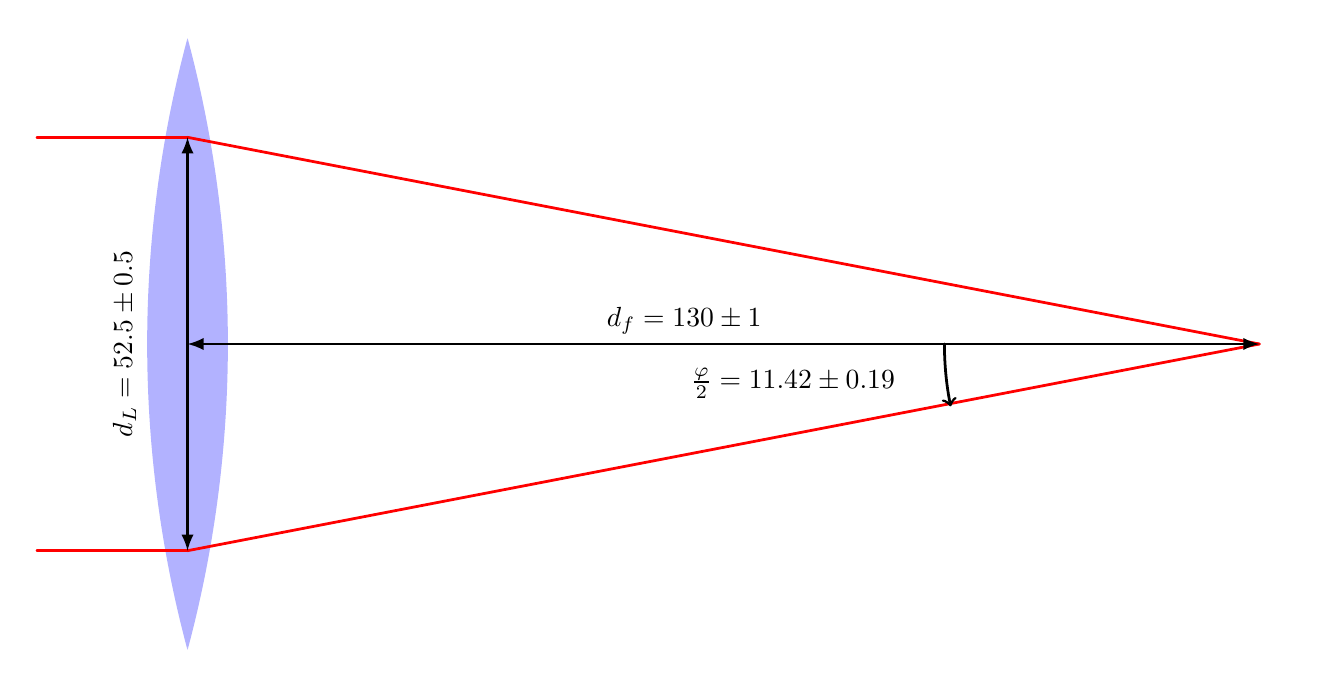
\begin{tikzpicture}
    \begin{scope}[x={(0mm,160mm)},y={(-40mm,40mm)},line width=1pt,cap=round]
        % bounding box
        \draw[white] (0mm,-40mm) rectangle (160mm,40mm);
        %\draw[-] (0mm,-30mm) -- (150mm,30mm);

        % Lens. Center: 20.125mm,0mm
        \fill[-,blue!30] (15mm,   0mm) -- (25.25mm,0mm) arc[start angle=0,  delta angle=15, radius=150mm] -- cycle;
        \fill[-,blue!30] (15mm,   0mm) -- (25.25mm,0mm) arc[start angle=0,  delta angle=-15,radius=150mm] -- cycle;
        \fill[-,blue!30] (25.25mm,0mm) -- (15mm,   0mm) arc[start angle=180,delta angle=15, radius=150mm] -- cycle;
        \fill[-,blue!30] (25.25mm,0mm) -- (15mm,   0mm) arc[start angle=180,delta angle=-15,radius=150mm] -- cycle;

        % incoming laser beams
        \draw[-,red] (1mm, 26.25mm) -- (20.125mm, 26.25mm);
        \draw[-,red] (1mm,-26.25mm) -- (20.125mm,-26.25mm);

        % outgoing laser beams
        \draw[-,red] (20.125mm, 26.25mm) -- (156.25mm,0mm);
        \draw[-,red] (20.125mm,-26.25mm) -- (156.25mm,0mm);

        % measurement arrow
        \draw[latex-latex,black] (20.125mm,0mm) -- (156.25mm,0mm);
        \draw[latex-latex,black] (20.125mm,-26.25mm) -- (20.125mm,26.25mm);
        \node[rotate=90] at (12.125mm,0mm) {$ d_L = \SI{52.5 \pm 0.5}{\milli\meter}$};
        \node at (83.2mm,3mm) {$ d_f = \SI{130 \pm 1}{\milli\meter}$};

        % angle arc
        \draw[->] (116.25mm,0mm) arc[start angle=180, delta angle=11.41, radius=40mm];
        \node at (97mm,-5mm) {$\frac{\varphi}{2} = \SI{11.42 \pm 0.19}{\degree}$};
    \end{scope}
\end{tikzpicture}
}
    \captionof{figure}{%
        Bestimmung des Schnittwinkels der  Laserstrahlen aus der Geometrie der
        Versuchsanordnung.  \emph{Beachte:} Da  diese Abbildung  prim\"ar  der
        Illustration  der Bestimmung  von  $\varphi$ und  nicht der  akkuraten
        Darstellung der Linse  dient, ist hier nicht das  gleiche Symbol f\"ur
        die Linse wie in der Versuchsanleitung benutzt worden.%
    }
    \label{fig:varphi}
\end{minipage}



% ---------------------------------------------------------------------------- $
\clearpage
\subsection{Str\"omungsgeschwindigkeit und Unsicherheiten}
\label{subsec:vUncert}
% ---------------------------------------------------------------------------- $


Gemessen  wurden  zwar  Frequenzen,  es  sollen  in  den  Regressionen  jedoch
direkt die zugeh\"origen Geschwindigkeiten  angegeben werden. Da diese Angaben
f\"ur  den  Rest  dieses  Kapitels  ben\"otigt  werden,  werden  zur  besseren
\"Ubersichtlichkeit  die  n\"otigen   Informationen  zur  Fehlerrechnung  hier
aufgef\"uhrt anstatt in einem separaten Kapitel im Nachhinein.

Die Flussgeschwindigkeiten k\"onnen mit der folgenden Formel ermittelt werden:

\begin{equation}
    %\begin{split}
        \label{eq:deltaF2}
        \Delta\,f = f_0 \cdot \frac{2 \cdot v}{c} \cdot \sin\left( \frac{\varphi}{2}\right)
                  = \frac{c}{\lambda_{Laser}} \cdot \frac{2 \cdot v}{c} \cdot \sin\left( \frac{\varphi}{2}\right)
                  = \frac{2 \cdot v}{\lambda_{Laser}} \cdot \sin\left( \frac{\varphi}{2}\right)
    %\end{split}
\end{equation}

Aufgel\"ost nach $v$ ergibt dies:
\begin{equation}
    \label{eq:vFromf}
    v = \frac{\Delta\,f \cdot \lambda_{Laser}}{2 \cdot \sin\left(\frac{\varphi}{2}\right)}
\end{equation}


\begin{conditions}
    v               & Flussgeschwindigkeit des Streuteilchens \\
    \Delta\,f       & Gemessene Streufrequenz                 \\
    \lambda_{Laser} & Wellenl\"ange des Lasers                \\
    \varphi         & Kreuzungswinkel der Laserstrahlen (\SI{22.8 \pm 0.4}{\degree} gem\"ass vorigem Abschnitt) \\
\end{conditions}

Es  sind  hier   sowohl  Unsicherheiten  im  Winkel  $\varphi$   wie  auch  in
der  gemessenen  Frequenz  vorhanden. Somit   ist  f\"ur  die  Bestimmung  der
Unsicherheit  der  Teilchengeschwindigkeit   die  Verwendung  des  Gauss'schen
Fehlerfortpflanzungsgesetzes erforderlich. Zur Erinnerung:

\begin{equation}
    \label{eq:Gauss}
    %\begin{split}
    s_{\overline{R}} = \sqrt{ \left( \frac{\partial R}{\partial x} \biggr\rvert_{\overline{R}} \cdot s_{\overline{x}}\right)^2
                            + \left( \frac{\partial R}{\partial y} \biggr\rvert_{\overline{R}} \cdot s_{\overline{y}}\right)^2
                            + \left( \frac{\partial R}{\partial z} \biggr\rvert_{\overline{R}} \cdot s_{\overline{z}}\right)^2
                            + ... }
    %\end{split}
\end{equation}

Angewandt auf die Formel der Teilchengeschwindigkeit:

\begin{equation}
    \label{eq:gauss:teilchen}
    \begin{split}
        s_{\overline{v}} = \sqrt{ \left( \frac{\partial v}{\partial f}       \biggr\rvert_{\overline{v}}       \cdot s_{\overline{f}}       \right)^2
                                + \left( \frac{\partial v}{\partial \varphi} \biggr\rvert_{\overline{\varphi}} \cdot s_{\overline{\varphi}} \right)^2
                                } \\
    \end{split}
\end{equation}

Mit:
\begin{align}
    \label{eq:partials}
    \frac{\partial v}{\partial f}       &= \frac{\lambda}{2 \cdot \sin \left( \frac{\varphi}{2} \right) } \\
    \frac{\partial v}{\partial \varphi} &= \frac{-f \cdot \lambda \cdot \cos\left(\frac{\varphi}{2}\right)}{4 \cdot \sin^2\left(\frac{\varphi}{2}\right)}
\end{align}

Ergibt sich somit:
\begin{equation}
    \label{eq:gauss:teilchen:eingesetzt}
    s_{\overline{v}} = \sqrt{ \left( \frac{\lambda}                                                    {2 \cdot \sin  \left( \frac{\varphi}{2} \right)} \biggr\rvert_{\overline{v}}       \cdot s_{\overline{f}}       \right)^2
                            + \left( \frac{-f \cdot \lambda \cdot \cos\left( \frac{\varphi}{2} \right)}{4 \cdot \sin^2\left( \frac{\varphi}{2} \right)} \biggr\rvert_{\overline{\varphi}} \cdot s_{\overline{\varphi}} \right)^2
                            }
\end{equation}

Formel   \ref{eq:gauss:teilchen:eingesetzt}  und   die  Messwerte   wurden  in
Python-Scripts   ausgewertet,  die   in  Anhang   \ref{app:python}  ab   Seite
\pageref{app:python} zu finden sind.



% ---------------------------------------------------------------------------- $
\clearpage
\subsection{Str\"omungsgeschwindigkeit auf Achse der Messleitung}
\label{subsec:achse}
% ---------------------------------------------------------------------------- $


Das   zu   diesem   Abschnitt   ge\"ohrende  Python-Script   ist   in   Anhang
\ref{app:python:rohrmitte}   auf   Seite   \pageref{app:python:rohrmitte}   zu
finden. Die  resultierenden  Flussgeschwindigkeiten mit  ihren  Unsicherheiten
sind in Tabelle \ref{tab:rohrmitte} zu finden.

\begin{table}[h!t]
    \centering
    \caption{Messwerte f\"ur verschiedene Durchflussraten in Rohrmitte}
    \label{tab:rohrmitte}
    \begin{tabular}{SSSSSS}
        \toprule
        {$\dot{V}$ (\si{\liter\per\minute})}
        & {$f_{low}$ (\si{\kilo\hertz})}
        & {$f_{high}$ (\si{\kilo\hertz})}
        & {$\overline{f}$ (\si{\kilo\hertz})}
        & {$s_{\overline{f}}$ (\si{\kilo\hertz})}
        & {$v$ (\si{\centi\meter\per\second})}
        \\

        \midrule

        0.5
        & 7.07
        & 7.71
        & 7.39
        & 0.32
        & 1.18 \pm 0.05
        \\

        1.01
        & 13.43
        & 14.38
        & 13.905
        & 0.475
        & 2.22 \pm 0.08
        \\

        1.52
        & 17.59
        & 19.77
        & 18.68
        & 1.09
        & 2.99 \pm 0.18
        \\

        2.02
        & 23.19
        & 25.32
        & 24.255
        & 1.065
        & 3.88 \pm 0.18
        \\

        2.5
        & 26.66
        & 30.29
        & 28.475
        & 1.815
        & 4.55 \pm 0.30
        \\

        3.0
        & 30.18
        & 35.09
        & 32.585
        & 2.505
        & 5.22 \pm 0.40
        \\

        3.5
        & 34.85
        & 39.3
        & 37.075
        & 2.225
        & 5.93 \pm 0.37
        \\

        4.0
        & 36.21
        & 43.12
        & 39.665
        & 3.455
        & 6.34 \pm 0.56
        \\

        4.5
        & 40.95
        & 49.48
        & 45.215
        & 4.265
        & 7.23 \pm 0.69
        \\

        5.0
        & 45.51
        & 52.75
        & 49.13
        & 3.62
        & 7.86 \pm 0.59
        \\

        5.5
        & 51.34
        & 58.30
        & 54.82
        & 3.48
        & 8.77 \pm 0.57
        \\

        6.0
        & 57.16
        & 61.91
        & 59.535
        & 2.375
        & 9.52 \pm 0.41
        \\

        6.5
        & 60.78
        & 70.84
        & 65.81
        & 5.03
        &10.52 \pm 0.82
        \\

        7.0
        & 64.44
        & 72.48
        & 68.46
        & 4.02
        &10.95 \pm 0.67
        \\

        7.5
        & 67.12
        & 77.42
        & 72.27
        & 5.15
        &11.56 \pm 0.85
        \\

        \bottomrule
    \end{tabular}
\end{table}

Die Werte aus  der letzten Spalte wurden anschliessend  in QtiPlot eingegeben,
zusammen mit den zugeh\"origen Durchflusswerten.

Wie      im     Abschnitt      \ref{subsubsec:laminarVsTurb}     ab      Seite
\pageref{subsubsec:laminarVsTurb} erw\"ahnt, liegt  die kritische Reynoldszahl
f\"ur den Fall einer zylindrischen Messleitung bei ungef\"ahr $2000$. Will man
die f\"ur unsere  Anordnung zugeh\"orige Str\"omungsgeschwindigkeit bestimmen,
l\"ost  man zuerst  Formel \ref{eq:reynolds}  von Seite  \pageref{eq:reynolds}
nach der mittleren Str\"omungsgeschwindigkeit auf, und erh\"alt:

\begin{equation}
    \label{eq:v:reynolds_krit}
    v_{\mathrm{m,krit}} = \frac{\mathit{Re_{\mathrm{krit}}} \cdot \eta}{\rho \cdot L} = \frac{\mathit{Re_{\mathrm{krit}}} \cdot \eta}{\rho \cdot 2R} = \SI{0.05}{\meter\per\second}
\end{equation}

\begin{conditions}
    \mathit{Re_{\mathrm{krit}}} & 2000 \\
    \eta                        & \SI{1}{\milli\pascal\second} \\
    \rho                        & \SI{1000}{\kilo\gram\per\cubic\meter} \\
    R                           & \SI{20}{\milli\meter} \\
\end{conditions}

Da  $v_{\mathrm{m}} =  \frac{\dot{V}}{A}$,  kann daraus  nun die  zugeh\"orige
Durchflussrate bestimmt werden:

\begin{equation}
    \label{eq:Q:reynolds_krit}
    \dot{V}_{\mathrm{krit}} = v_{\mathrm{m,krit}} \cdot A = \SI{0.000063}{\cubic\meter\per\second} \approx \SI{3.78}{\liter\per\minute}
\end{equation}

\begin{samepage}
\begin{figure}[h!t]
    \centering
    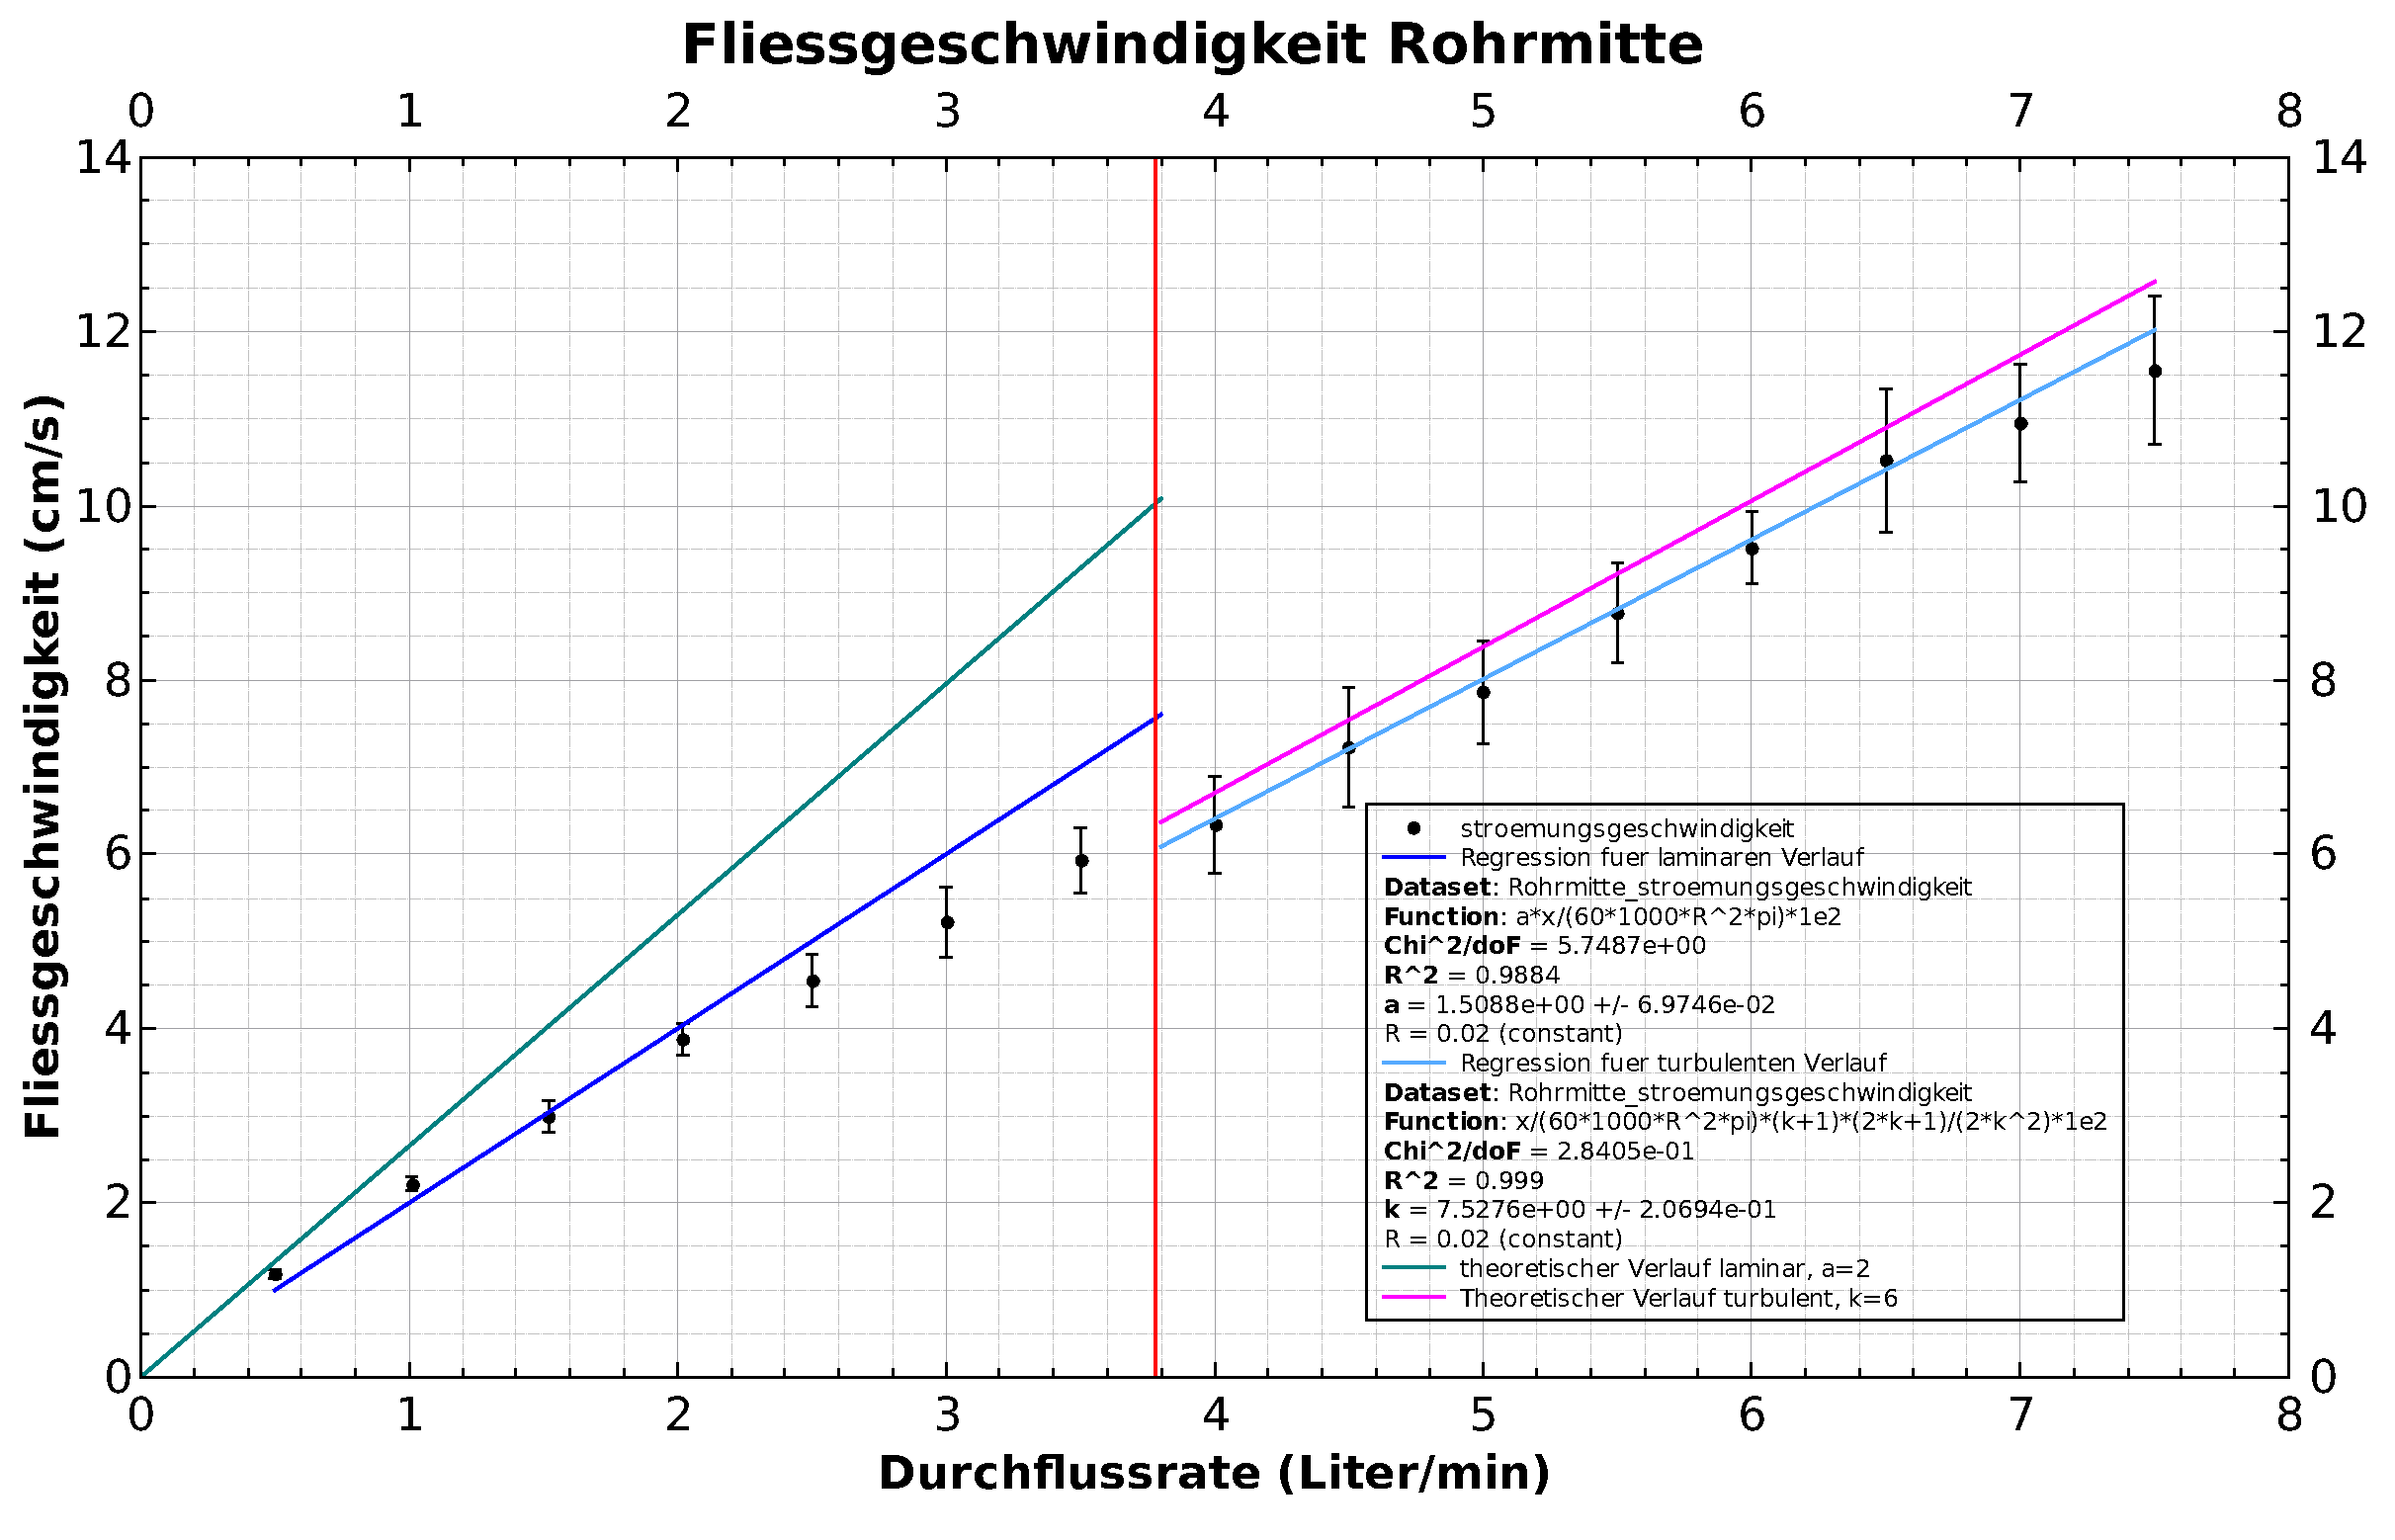
\includegraphics[width=\textwidth]{images/rohrmitte.pdf}
    \captionsetup{singlelinecheck=off}
    \caption[foo bar]{%
        Verlauf    von     Durchflussrate    und    Str\"omungsgeschwindigkeit
        in     der     Rohrmitte. Es sind folgende Linien eingezeichnet:
        \begin{itemize}
            \item
                rot: Durchfluss, welcher der kritischen Reynoldszahl von ca. \num{2000} entspricht gem\"ass Gleichung \ref{eq:Q:reynolds_krit}
            \item
                dunkel-cyan: theoretischer Verlauf der maximalen Str\"omungsgeschwindigkeit im laminaren Fall: $v_{\mathrm{max, laminar}} = 2 \cdot \frac{\dot{V}}{A}$
            \item
                blau: Regression f\"ur den Verlauf der maximalen Str\"omungsgeschwindigkeit im laminaren Fall: $v_{\mathrm{max, laminar}} = a \cdot \frac{\dot{V}}{A}$, mit Regressionsparameter $a = 1.5088 \pm 0.069746$
            \item
                magenta: theoretischer Verlauf der maximalen Str\"omungsgeschwindigkeit im turbulenten Fall: $v_{\mathrm{max, turbulent}} = \frac{\dot{V}}{A} \cdot \frac{(k + 1) \cdot (2k + 1)}{2 \cdot k^2}$, mit $k = 6$
            \item
                cyan: Regression f\"ur die maximale Str\"omungsgeschwindigkeit im turbulenten Fall: $v_{\mathrm{max, turbulent}} = \frac{\dot{V}}{A} \cdot \frac{(k + 1) \cdot (2k + 1)}{2 \cdot k^2}$, mit $k = 7.5276 \pm 0.20694$ als Regressionsparameter
        \end{itemize}
    }
    \label{fig:flowspeed:middle}
\end{figure}

Abbildung  \ref{fig:flowspeed:middle}  stellt  die  Messpunkte  der  maximalen
Str\"omungsgeschwindigkeit  (Rohrmitte) in  Abh\"angigkeit der  Durchflussrate
$\dot{V}$ dar.   Vergleicht man  die dunkel-cyan-farbene  Linie (theoretischer
Verlauf  der  maximalen  Flussgeschwindigkeit im  laminaren  Bereich  gem\"ass
$v_{\mathrm{max}} =  2 \cdot \frac{\dot{V}}{A}$)  mit den Messungen,  kann man
erkennen, dass  die Messungen bei steigender  Durchflussrate vom theoretischen
Verlauf abzuweichen beginnen.

Die    Ursache   daf\"ur    liegt   in    der   zu    kurzen   Einlaufstrecke,
wie    in    Abbildung    \ref{fig:ausbildungLaminareStromung}    auf    Seite
\pageref{fig:ausbildungLaminareStromung}    dargestellt. Je     h\"oher    der
Durchfluss,  um  so  gr\"osser   die  Abweichung  zwischen  theoretischem  und
effektivem   Wert,  wie   auch  in   Abbildung  \ref{fig:einlauf}   auf  Seite
\pageref{fig:einlauf} erkennbar.

Auch beim  theoretischen Verlauf im  turbulenten Bereich liegen  die Messwerte
etwas unter den theoretisch erwarteten Werten, jedoch nicht ganz so stark. Ich
erkl\"are dies  damit, dass das  turbulente Profil eben  nicht parabelf\"ormig
ist,  sondern   gegen  die   Mitte  der  Leitung   nur  noch   relative  flach
ansteigt. Somit macht sich  die zu kurze Einlaufstrecke  vermutlich nicht mehr
so stark bemerkbar

Aus Neugier wurden f\"ur die beiden Bereiche (laminar, turbulent) jeweils noch
eine gewichtete Regression durchgef\"uhrt,  einmal mit einem Koeffizienten $a$
als Regressionsparameter (im laminaren Fall),  und im turbulenten Fall mit $k$
als Regressionsparameter. Als Resultat lieferte QtiPlot:

\begin{align}
    \label{eq:rohrmitte:regressionresults}
    \text{Regressions-Funktion: } v_{\mathrm{max, laminar}}     &= a \cdot \frac{\dot{V}}{A} \\
    \text{Resultat: }                                                  a &= 1.5088 \pm 0.069746 \\
    \text{Regressions-Funktion: } v_{\mathrm{max, turbulent}} &= \frac{\dot{V}}{A} \cdot \frac{(k + 1) \cdot (2k + 1)}{2 \cdot k^2} \\
    \text{Resultat: }                                                  k &= 7.5276 \pm 0.20694
\end{align}
\end{samepage}

Da sich  $a$ mit zunehmendem  Durchfluss eigentlich \"andert  (siehe Abbildung
\ref{fig:einlauf}, Seite \pageref{fig:einlauf}\footnotemark[2]), sollte dieses
Regressionsresultat nat\"urlich nicht einfach in eine Gleichung eingesetzt und
verwendet werden. Die  Regression wurde  aber nicht durchgef\"uhrt,  um diesen
Parameter  m\"oglichst genau  zu  bestimmen, sondern  um zu  veranschaulichen,
dass  er  doch  recht  betr\"achtlich vom  theoretischen  Wert  eines  perfekt
parabolischen Profils abweichen kann, was meines Erachtens gelungen ist.

Der   Wert    f\"ur   $k$    ist   \"uber    dem   theoretischen    Wert   von
\num{6}\footnotemark[3]. Dies  deckt sich  jedoch zumindest  einigermassen mit
den  Ergebnissen der  Regression beim  turbulenten Str\"omungsprofil,  wie wir
sp\"ater sehen werden.

\footnotetext[2]{%
    Der  in der  Regression bestimmte  Parameter $a$  taucht in  der Abbildung
    nicht direkt  auf, ist jedoch  an das Verh\"altnis  von $v_{\mathrm{max}}$
    und  $v_{\mathrm{m}}$  gebunden, weshalb  die  Abbildung  und der  in  der
    Regression bestimte Parameter trotzdem eng zusammenh\"angen.
}

\footnotetext[3]{%
    Wie in  den Arbeitsgrundlagen angemerkt,  variiert $k$ bei  \"Anderung der
    Reynoldszahl im  Bereich von  mehreren Zehnerpotenzen lediglich  um einige
    Inkremente, daher  wird $k$  approximativ \"uber den  betrachteten Bereich
    zur Veranschaulichung in diesem Fall als konstant betrachtet.
}

% ---------------------------------------------------------------------------- $
\clearpage
\subsection{Str\"omungsprofil im laminaren Fall}
\label{subsec:profil:laminar}
% ---------------------------------------------------------------------------- $

Das  Vorgehen  zur Bestimmung  der  Str\"omungsgeschwindigkeit  ist in  diesem
Falle  identisch. Der  Unterschied  zur   obigen  Messung  liegt  darin,  dass
die  Durchflussrate   fixiert  war   und  die  Position   variiert  wurde. Das
Python-Script f\"ur die Resultate aus  Tabelle \ref{tab:laminar} ist in Anhang
\ref{app:python:laminar} auf Seite \pageref{app:python:laminar} zu finden.

\begin{table}[h!t]
    \centering
    \caption{Messwerte f\"ur Str\"omungsprofil im laminaren Fall ($\dot{V} = \SI{0.56}{\liter\per\minute}$)}
    \label{tab:laminar}
    \begin{tabular}{SSSSSS}
        \toprule
        {Position (\si{\milli\meter})}
        & {$f_{low}$ (\si{\kilo\hertz})}
        & {$f_{high}$ (\si{\kilo\hertz})}
        & {$\overline{f}$ (\si{\kilo\hertz})}
        & {$s_{\overline{f}}$ (\si{\kilo\hertz})}
        & {$v$ (\si{\centi\meter\per\second})}
        \\

        \midrule

        -13.33
        & 4.51
        & 5.20
        & 4.885
        & 0.345
        & 0.8   \pm  0.1
        \\

        -12.00
        & 5.35
        & 5.93
        & 5.64
        & 0.29
        & 0.9   \pm  0.05
        \\

        -10.67
        & 5.93
        & 6.67
        & 6.30
        & 0.37
        & 1.0   \pm  0.1
        \\

        -9.33
        & 6.72
        & 7.27
        & 6.995
        & 0.275
        & 1.1   \pm  0.05
        \\

        -8
        & 7.31
        & 7.95
        & 7.63
        & 0.32
        & 1.2   \pm  0.1
        \\

        -5.33
        & 8.19
        & 8.65
        & 8.42
        & 0.23
        & 1.3   \pm  0.04
        \\

        -2.67
        & 8.25
        & 8.68
        & 8.465
        & 0.215
        & 1.35  \pm  0.04
        \\

        0
        & 8.39
        & 8.88
        & 8.635
        & 0.245
        & 1.38  \pm  0.05
        \\

        2.67
        & 8.16
        & 8.54
        & 8.35
        & 0.19
        & 1.33  \pm  0.04
        \\

        5.33
        & 7.80
        & 8.36
        & 8.08
        & 0.28
        & 1.29  \pm  0.05
        \\

        8.0
        & 6.87
        & 7.43
        & 7.15
        & 0.28
        & 1.14  \pm  0.05
        \\

        9.33
        & 6.76
        & 7.34
        & 7.05
        & 0.29
        & 1.13  \pm  0.05
        \\

        10.67
        & 6.29
        & 7.02
        & 6.655
        & 0.365
        & 1.06  \pm  0.1
        \\

        12.0
        & 5.76
        & 6.37
        & 6.065
        & 0.305
        & 0.98  \pm  0.1
        \\

        13.33
        & 5.29
        & 5.84
        & 5.565
        & 0.275
        & 0.89  \pm  0.05
        \\

        14.67
        & 4.53
        & 5.18
        & 4.855
        & 0.325
        & 0.78  \pm  0.1
        \\

        16.00
        & 3.69
        & 4.41
        & 4.05
        & 0.36
        & 0.65  \pm  0.1
        \\

        17.33
        & 2.81
        & 3.42
        & 3.115
        & 0.305
        & 0.5   \pm  0.05
        \\

        \bottomrule
    \end{tabular}
\end{table}

\clearpage
\begin{samepage}
Als Formel  zur Regression  wurde Gleichung \ref{eq:laminarprofile}  von Seite
\pageref{eq:laminarprofile} benutzt. Fit-Variable war $v_{\mathrm{max}}$.

\begin{figure}[h!t]
    \centering
    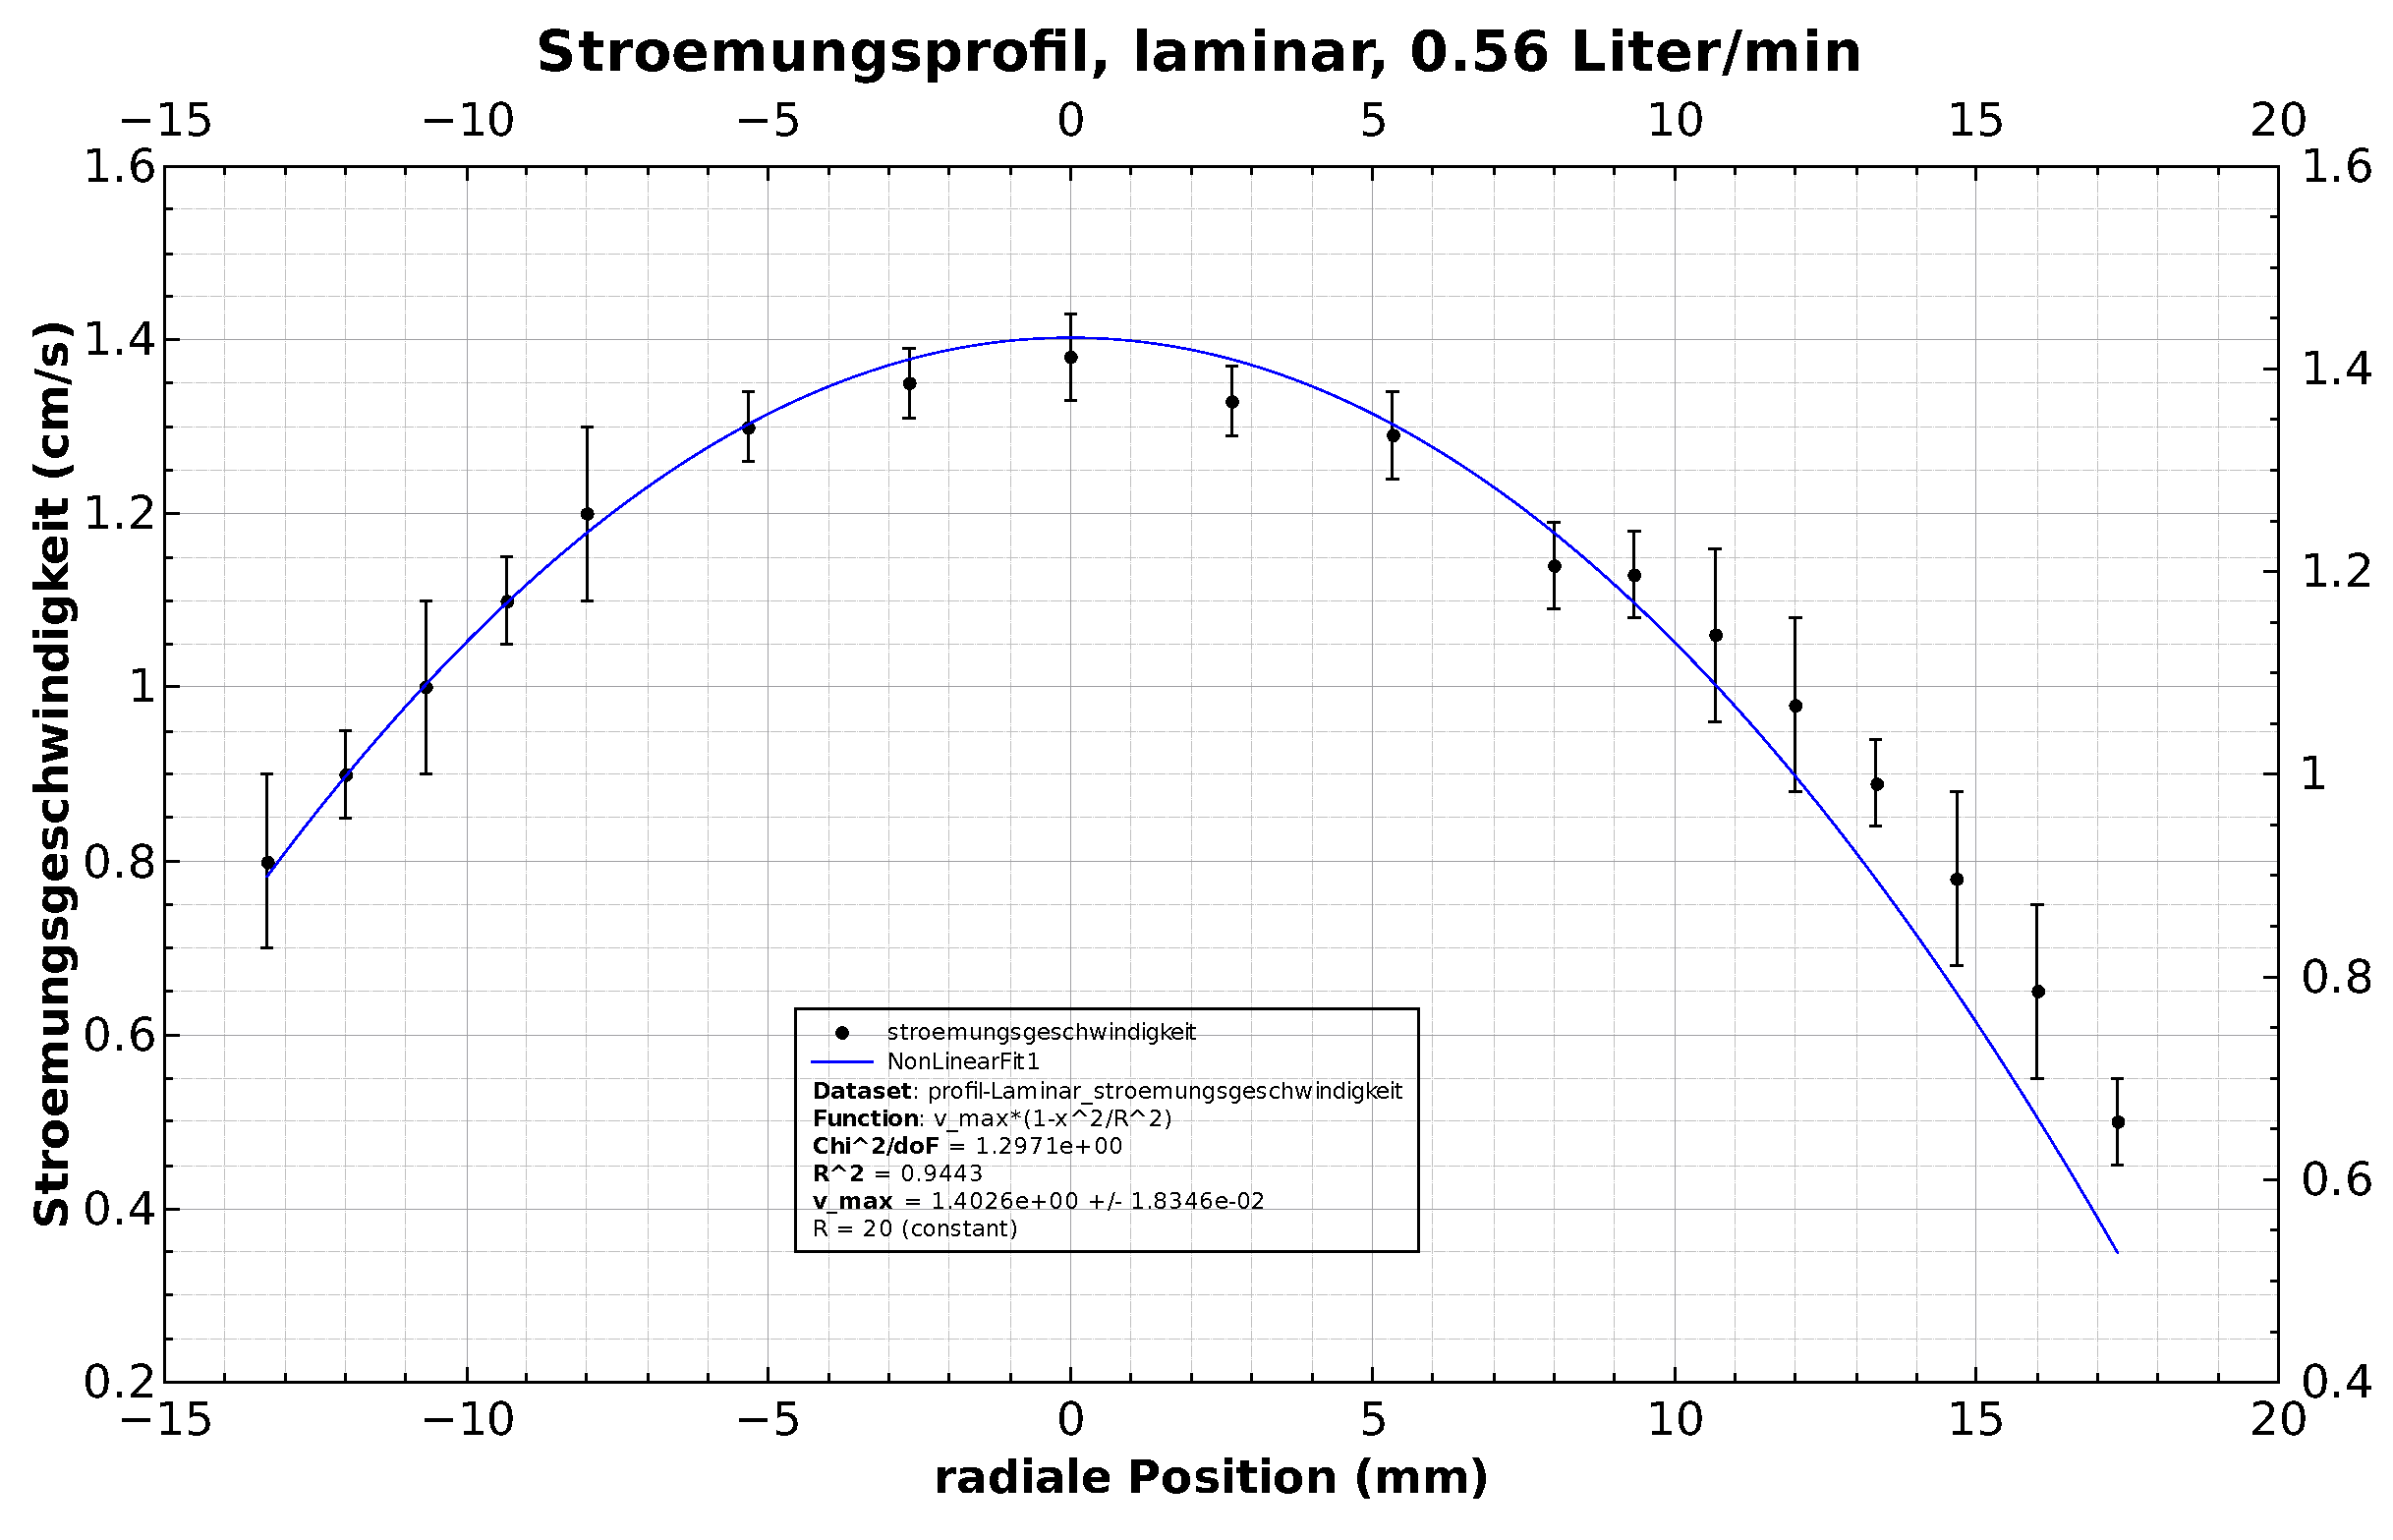
\includegraphics[width=\textwidth]{images/profil-laminar.pdf}
    \caption{Gewichtete Regression an die Messpunkte des Str\"omungsprofils im laminaren Fall}
    \label{fig:profile:laminar}
\end{figure}

Die  Regression  stimmt  recht  gut mit  den  Messpunkten  \"uberein. Es  kann
gesehen  werden, dass  die  maximale Geschwindigkeit  in  der Rohrmitte  nicht
ganz an  den Scheitelpunkt  der Parabel heranreicht. Die  Begr\"undung daf\"ur
liegt  darin, dass  die Messleitung  nicht  gen\"ugend lang  ist, um  wirklich
einen  vollst\"andig  laminaren  Fluss   herausbilden  zu  konnen  (zu  kleine
Einlaufl\"ange), wie auch im  vorigen Abschnitt erw\"ahnt. Gegen die Rohrmitte
wird  das Str\"omungsprofil  dadurch   gegen\"uber  der theoretischen  Parabel
abgeflacht. Siehe  dazu auch  Abbildungen \ref{fig:ausbildungLaminareStromung}
und  \ref{fig:einlauf}   auf  Seiten  \pageref{fig:ausbildungLaminareStromung}
respektive \pageref{fig:einlauf} und die zugeh\"origen Anmerkungen.

\begin{equation}
    \label{eq:profile:laminar:regression:results:vmax}
    v_{\mathrm{max}} = \SI{1.4026 \pm 0.018346}{\centi\meter\per\second}
\end{equation}

Es sei hier noch betont, dass eine \emph{gewichtete} Regression gemacht wurde.
\end{samepage}

% ---------------------------------------------------------------------------- $
\clearpage
\subsection{Str\"omungsprofil im turbulenten Fall}
\label{subsec:profil:turbulent}
% ---------------------------------------------------------------------------- $

Das Vorgehen ist  in diesem Falle identisch wie im  vorherigen Abschnitt.  Das
Python-Script  f\"ur  die Resultate  aus  Tabelle  \ref{tab:turbulent} ist  in
Anhang  \ref{app:python:laminar} auf  Seite \pageref{app:python:turbulent}  zu
finden.

Aus  Zeitgr\"unden  wurden  f\"ur  das  turbulente  Str\"omungsprofil  weniger
Messungen gemacht als f\"ur das laminare.

\begin{table}[h!t]
    \centering
    \caption{Messwerte f\"ur Str\"omungsprofil im turbulenten Fall ($\dot{V} = \SI{7}{\liter\per\minute}$)}
    \label{tab:turbulent}
    \begin{tabular}{SSSSSS}
        \toprule
        {Position (\si{\milli\meter})}
        & {$f_{low}$ (\si{\kilo\hertz})}
        & {$f_{high}$ (\si{\kilo\hertz})}
        & {$\overline{f}$ (\si{\kilo\hertz})}
        & {$s_{\overline{f}}$ (\si{\kilo\hertz})}
        & {$v$ (\si{\centi\meter\per\second})}
        \\

        \midrule

        -10.67
        & 49.59
        & 63.13
        & 56.36
        & 6.77
        & 9.0 \pm 1.1
        \\

        -8
        & 53.77
        & 67.77
        & 60.77
        & 7.0
        & 9.7 \pm 1.1
        \\

        -5.33
        & 57.74
        & 69.51
        & 63.625
        & 5.885
        &10.2 \pm 1.0
        \\

        -2.67
        & 54.17
        & 68.96
        & 61.596
        & 7.395
        & 9.8 \pm 1.2
        \\

        0
        & 63.41
        & 71.31
        & 67,36
        & 3.95
        &10.8 \pm 0.7
        \\

        2.67
        & 61.58
        & 74.02
        & 67.8
        & 6.22
        &10.8 \pm 1.0
        \\

        5.33
        & 62.86
        & 70.18
        & 66.52
        & 3.66
        &10.6 \pm 0.6
        \\

        8.0
        & 60.6
        & 69.23
        & 64.915
        & 4.315
        &10.4 \pm 0.7
        \\

        10.67
        & 55.42
        & 68.84
        & 62.13
        & 6.71
        & 9.9 \pm 1.1
        \\

        12.0
        & 54.53
        & 71.46
        & 62.995
        & 8.465
        &10.1 \pm 1.4
        \\

        13.33
        & 48.01
        & 67.83
        & 57.92
        & 9.91
        & 9.3 \pm 1.6
        \\

        14.67
        & 47.52
        & 66.09
        & 56.805
        & 9.285
        & 9.1 \pm 1.5
        \\

        16.00
        & 44.77
        & 65.85
        & 55.31
        & 10.54
        & 8.8 \pm 1.7
        \\

        17.33
        & 38.98
        & 66.98
        & 52.98
        & 14
        & 8.5 \pm 2.2
        \\

        \bottomrule
    \end{tabular}
\end{table}

Zur Regression and diese Daten wurde Gleichung \ref{eq:potenzgesetz} von Seite
\pageref{eq:potenzgesetz} herangezogen, mit einer kleinen Modifikation. Da die
Funktion in  der gegebenen Form ungerade  ist und somit f\"ur  negative Radien
nicht das gew\"unschte Ergebnis liefert,  wurde zur Regression noch ein Betrag
eingebaut:

\begin{equation}
    \label{eq:potenzgesetz:abs}
    v(r) = v_{\mathrm{max}} \cdot \left( 1 - \abs*{\frac{r}{R}} \right)^{\frac{1}{k}}
\end{equation}

\clearpage
\begin{samepage}
\begin{figure}[h!t]
    \centering
    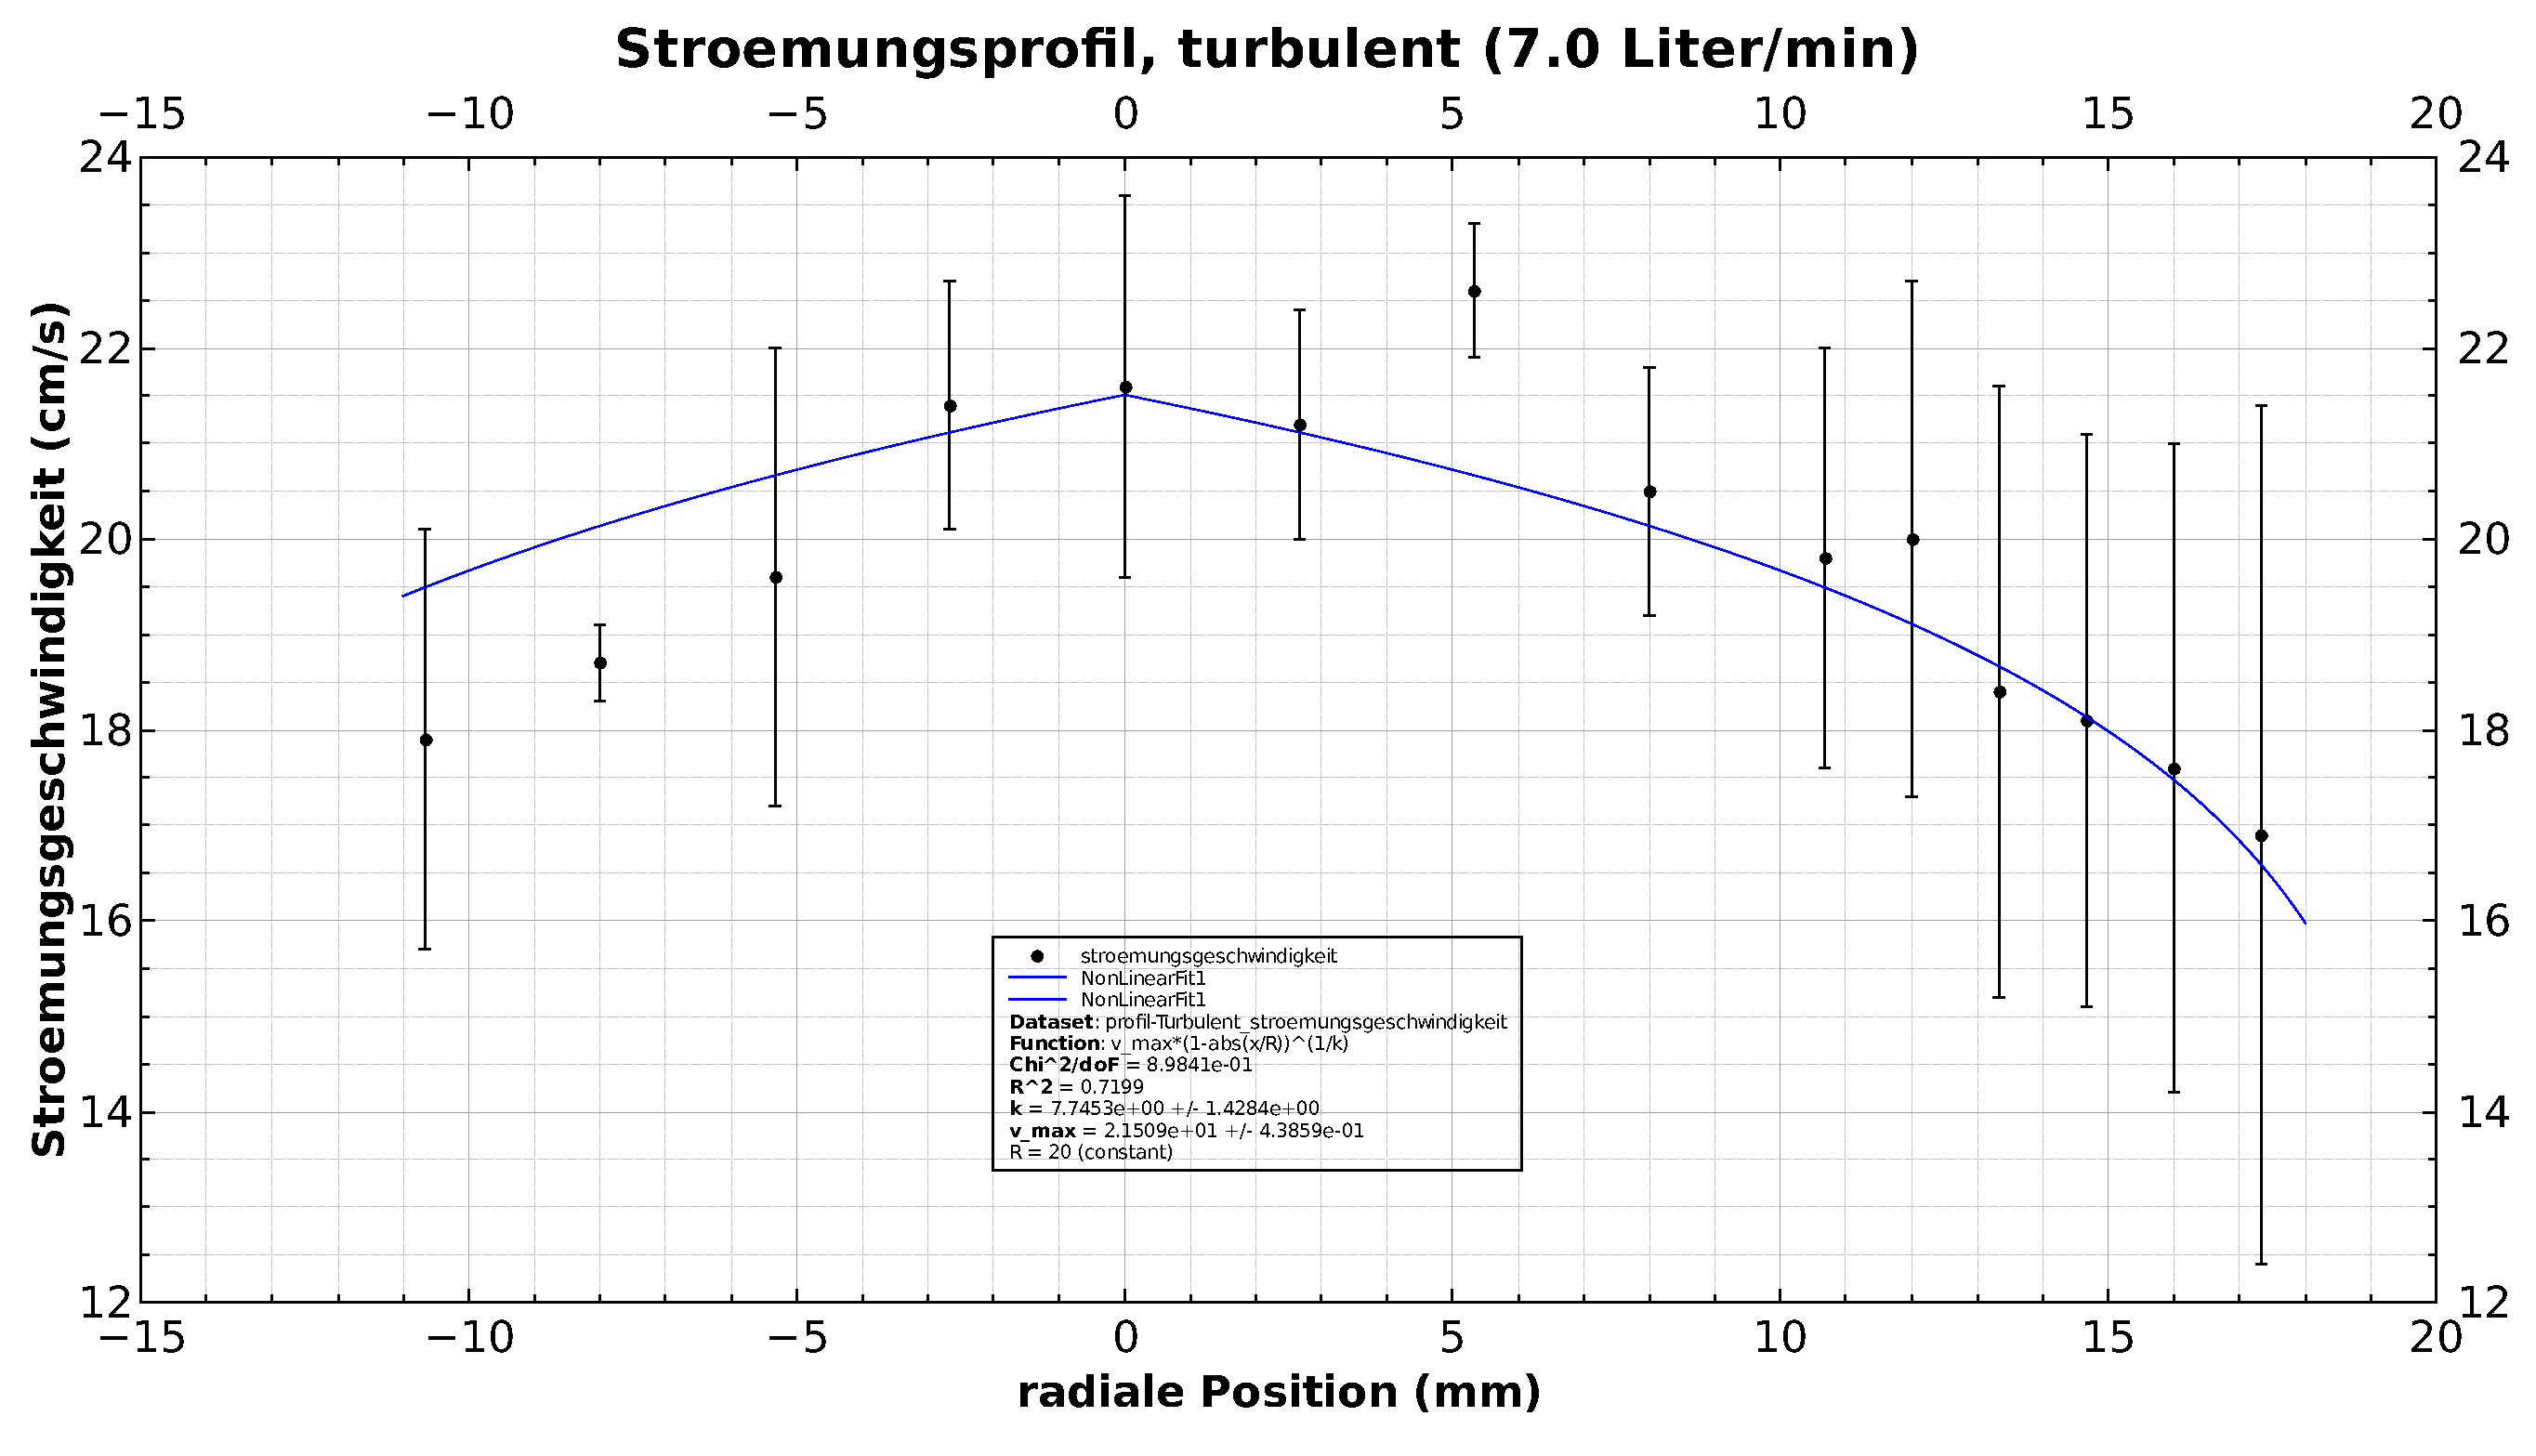
\includegraphics[width=\textwidth]{images/profil-turbulent.pdf}
    \caption{Gewichtete Regression f\"ur das Str\"omungsprofil im turbulenten Fall.}
    \label{fig:profile:turb}
\end{figure}

Regressionsparameter  waren $k$  und $v_{\mathrm{max}}$. Als  Ergebnis liefert
QtiPlot:

\begin{align}
    \label{eq:profile:turb:regression:results:k}
    k &= 7.8876 \pm 1.5642
    \\
    \label{eq:profile:turb:regression:results:vmax}
    v_{\mathrm{max}} &= \SI{10.793 \pm 0.1572}{\centi\meter\per\second}
\end{align}

Wie man  in Tabelle  \ref{tab:turbulent} und  Abbildung \ref{fig:profile:turb}
unschwer erkennen kann, sind die Unsicherheiten bei den Werten teilweise recht
gross. Ich erkl\"are  mir dies dadurch, dass  das turbulente Str\"omungsprofil
eben  nicht  so  sauber  ausgepr\"agt   ist,  wie  es  die  Vereinfachung  aus
Abbildung \ref{fig:turbProfile} von Seite \pageref{fig:turbProfile} allenfalls
Glauben  macht. Betrachtet   man  Abbildung   \ref{fig:turbulentesProfil}  auf
Seite  \pageref{fig:turbulentesProfil},   so  kann   man  erkennen,   dass  in
einer  turbulenten  Str\"omung  grob   gesagt  einiges  Chaos  herrscht  (oder
eben: Turbulenzen). Die   Str\"omungsgeschwindigkeit  (und   somit  auch   die
beobachteten  Frequenzen)  kann  deshalb  am  gleichen  Ort  \"uber  die  Zeit
bedeutend  variieren, auch  wenn  sie gemittelt  als  ein Profil  angen\"ahert
werden kann.

Betrachtet man den Verlauf der Regression in Abbildung \ref{fig:profile:turb},
kann   zumindest   auf  der   rechten   Seite   jedoch  eine   ganz   passable
\"Ubereinstimmung zwischen  Messungen und Regression festgestellt  werden, und
sowohl der Wert f\"ur $k$ wie auch f\"ur $v_{\mathrm{max}}$ sind einigermassen
plausibel ($k$ ist  h\"oher als erwartet; gem\"ass Versuchsanleitung  ist $k =
6$ f\"ur $\mathit{Re}  \approx 4000$, aber die  Gr\"ossenordnung scheint nicht
schlecht zu stimmen).

Auch hier wurde eine gewichtete Regression durchgef\"uhrt.
\end{samepage}
